%\section{To-Do List}
%
%\begin{itemize}
%\item General: Rewrite the paper to focus less on methodology and more on transformations and refactoring
%\item Add a section about dynamic trace-based pattern discovery that we do
%\item Shorten out the Software Restoration section
%\item Have two section on refactoring:
%  \begin{itemize}
%  \item One with ``lower-level'' refactorings, eliminating \lstinline{pthread_create}, locks etc.
%    \item One with ``high-level'' refactorings to eliminate patterns
%    \end{itemize}
%  \item Look at the PARSEC benchmark suite and see what applications we can refactor
%  \item Look at the SE metrics and decide which ones to use in evaluation
%    \item Evaluate the technique with chosen metrics and chosen use cases
% \end{itemize}

\section{Introduction}

Parallel patterns are a well-established high-level parallel programming model for producing portable, maintainable, adaptive, and efficient parallel code. They have been endorsed by some of the biggest IT companies, such as Intel and Microsoft, who have developed their own parallel pattern libraries (Intel TBB~\cite{DBLP:reference/parallel/X11pz}, Microsoft PPL, etc.) A standard way to use these libraries is to start with a sequential code base, identifying in it the portions of code that are amenable to parallelisation, together with the exact parallel pattern to be applied.  Then instantiating the identified pattern at the identified location in the code, after possibly restructuring the code to accommodate the parallelism. 

%Figure~\ref{fig:matmult} shows an example of sequential and parallel patterned-code of Matrix Multiplication, one of the most common parallel benchmarks. 

%\begin{small}
%  \begin{lstlisting}[caption=Pthreads Matrix Multiplication\label{lst:matmult_seq}]
%double multiply_row_by_column (double **mat1, int row, double **mat2, int col)
%{
%  int k;
%  double sum=0;
%  for (k=0; k<dim; k++)
%    sum += mat1[row][k] * mat2[k][col];%

%  return sum;
%}

%void multiply_row_by_matrix (double **mat1, int row, double **mat2, double **res)
%{
%  for (int col=0; col<dim; col++)
%    res[row][col] = multiply_row_by_column (mat1, row, mat2, col);

%}

%static void * thread_func (void* arg)
%{
 % input_data *input = (input_data *)arg;
 % for (unsigned int i = input->row_start; i < input->row_end; i++) {
 %         multiply_row_by_matrix(a, i, b, res);
 % }

%  return (void *)0;
%}

%void matrix_muliply()
%{
%  pthread_attr_t attr;
%  int status;%

%  in = (input_data *) malloc (sizeof(input_data) * thread_count);
%  threads = (pthread_t *) malloc (sizeof(pthread_t) * thread_count);
  
%  status = pthread_attr_init(&attr);
%  if (status != 0)
%    std::cout << "Init attributes object" << std::endl;

%  int chunk_size = dim / thread_count;
%  int count = 0;

%  for (unsigned int thread_ind = 0; thread_ind < thread_count; thread_ind++) {
%    /* Setting some generic parameters for each thread */
%    in[thread_ind].row_start = count;
 %   in[thread_ind].row_end = count + chunk;
  %  count += chunk;

   % status = pthread_create(&threads[thread_ind], &attr, &thread_func, &in[thread_ind]);
%    if (status != 0)
 %     handle_error("Creating thread failed!");

 % }%
%}
 % \end{lstlisting}
  
%\end{small}

Sequential code gives the cleanest starting point for introduction of parallel patterns. There exists, however, a large base of \emph{legacy} code  that was parallelised using lower-level, mostly ad-hoc parallelisation methods and libraries, such as \emph{pthreads}~\cite{10.5555/263953}. This code is usually very hard to read and understand, is tailored to a specific parallelisation, and optimised for a specific architecture, effectively preventing alternative (and possibly better) parallelisations and limiting portability and adaptivity of the code. An even bigger problem, from the software engineering perspective, is the maintainability of the legacy-parallel code: commonly, the programmer who wrote it is the only one who can understand and maintain the code. This is due to both complexity of low-level threading libraries and the need for custom-built data structures, synchronisation mechanisms, and sometimes even thread/task scheduling implemented in the code. 
%
The benefits of using parallel patterns lie in a clear separation between sequential and parallel parts of the code and a high-level description of the underlying parallelism, making the patterned applications much easier to maintain, change, and adapt to new architectures. Common examples include \emph{farms} and \emph{pipelines}.
%
%\begin{itemize}
%	\item 
In a farm, a single computational worker is applied to a set of independent inputs. The parallelism arises from applying the worker to different input elements in parallel. 
%	\item 
%The pipeline pattern models a parallel pipeline. 
In a parallel pipeline, a sequence of functions, $f_{1}, f_{2}, ..., f_{m}$ are applied to a stream of independent inputs, $x_{1}, ..., x_{n}$ where the output of $f_{i}$ becomes the input to $f_{i+1}$; the parallelism arises from executing $f_{i+1}(f_{i}(...f_{1}(x_{k})...))$ in parallel with $f_{i}(f_{i-1}(...f_{1}(x_{k+1})...))$.
%\end{itemize}



%Legacy-parallel code, written in an ad-hoc way using low level parallel libraries such as \emph{pthreads}, is still very much present in various software repositories and projects. This code was usually developed by parallelism experts, before the libraries and programming models for structured parallelisation became popular. It is usually tailored to one specific target machine and architecture, and might use highly-customised parallelisation and associated data structures. This makes it very hard to maintain the code, an increasing important feature in software engineering, or to port it to new architectures. 
  
In this paper, we present a new methodology for the restoration of legacy-parallel code into an equivalent \emph{patterned} form, through application of a number of identified program transformations; the ultimate goal of which is to provide a semi-automatic way of converting legacy-parallel code into an equivalent patterned code, therefore increasing its maintainability, adaptivity, and portability 
%while keeping similar or, in some cases, even improving the performance. 
whilst either improving or maintaining performance.
%
This paper makes the following specific research contributions:
%
\begin{enumerate}
    \item we present a novel software restoration methodology for converting legacy-parallel applications into their structured (patterned) parallel equivalents;
    \item we present a new set of \emph{restoration} transformations that attempt to \emph{systematically}, \emph{i}) \emph{eliminate} pthread operations from legacy C/C++ programs; \emph{ii}) perform \emph{code repair}, fixing any bugs introduced in \emph{i}; and, \emph{iii}) \emph{reshape} code in preparation for parallel pattern introduction;
%    eliminate parallelism from the legacy-parallel \lstinline{pthreads} code, providing semi-automatic implementation of the first step of software restoration methodology;
    \item we evaluate these transformations on a set of benchmarks, demonstrating that removal of parallelism can allow us to manually derive structured parallel code that is comparable to the original legacy-parallel version in terms of performance, while being more portable, adaptive, and maintainable.
\end{enumerate}

%\section{Background} \label{sec:background}
%Legacy-parallel code, written in an ad-hoc way using low level parallel libraries such as \emph{pthreads}, is still very much present in various software repositories and projects. This code was usually developed by parallelism experts, before the libraries and programming models for structured parallelisation became popular. It is usually tailored to one specific target machine and architecture, and might use highly-customised parallelisation and associated data structures. This makes it very hard to maintain that code, an increasing important feature in software engineering, or to port it to new architectures. It would be ideal if we could transform every legacy-parallel application into a structured parallel programs, written using high-level parallel programming libraries. However, for this to be possible, it is necessary that a well-defined underlying pattern of parallelism actually exists in the code, which can be exploited by instances of patterns. This is not always the case. However, in substantial number of cases, the parallelism in the application is an instance of one of the common patterns, such as farm, pipeline, workpool or stencil. In these cases, it should be possible, automatically or semi-automatically, to \emph{replace} unstructured parallelism with its structured (patterned) equivalent.   

%It would be ideal if we could transform every legacy-parallel application into a structured parallel programs, written using high-level parallel programming libraries. However, for this to be possible, it is necessary that a well-defined underlying pattern of parallelism actually exists in the code, which can be exploited by instances of patterns. This is not always the case. However, in a substantial number of cases, the parallelism in the application is an instance of one of the common patterns, such as farm, pipeline, workpool or stencil. In these cases, it should be possible, automatically or semi-automatically, to \emph{replace} unstructured parallelism with its structured (patterned) equivalent.   

%\section{Parallel Patterns}\label{sec:background}
%\begin{itemize}
%\item What are parallel patterns
%\item Some common patterns
%  \item Benefits of using patterns
%  \item Relevant pattern libraries (Open MP, Intel TBB...)
%\end{itemize}

\noindent
%\emph{Parallel patterns} are a high-level abstraction for representing classes of computations that are similar in terms of their parallel structure, but different in terms of problem-specific operations. A typical example of a parallel pattern is a \emph{parallel map}, where the same operation is applied to a set of independent inputs in parallel. 
%%Regardless of whether the actual operation is, for example, multiplying a matrix by a vector, processing a pixel of an image or XX, the parallel structure of the computation will be the same. Parallel Patterns are typically implemented as library functions which handle creation, synchronisation and communication between the parallel threads, while the problem-specific (often sequential) computations are provided as the pattern parameters. 
%In this paper, we restrict ourselves to two classical parallel patterns, which we believe to be the most common. Note that the technique described in this paper can be further generalised to include the full tractable set of parallel patterns.
%\begin{itemize}
%    \item The farm pattern models a data parallel computation, where a single computational worker, $f$, is applied to a set of independent inputs, $x_{1}, ..., x_{n}$. The parallelism arises from applying the worker, $f$, to different input elements at the same time in parallel. 
%    \item The pipeline pattern models a parallel pipeline. Here, a sequence of functions, $f_{1}, f_{2}, ..., f_{m}$ are applied to a stream on independent inputs, $x_{1}, ..., x_{n}$. The output of $f_{i}$ becomes the input to $f_{i+1}$, so that the parallelism arises from executing $f_{i+1}(f_{i}(...f_{1}(x_{k})...))$ in parallel with $f_{i}(f_{i-1}(...f_{1}(x_{k+1})...))$.
%\end{itemize}
%
%The benefits of using parallel patterns lie in clear separation between sequential and parallel parts of the code and high-level description of the underlying parallelism, which makes the patterned applications much easier to maintain, change and adapt to new architectures. 
%For these reasons, they have been endorsed by most of the top IT companies, who have their own pattern libraries, such as Microsoft PPL~\cite{ppl} and Intel Thread Building Blocks~\cite{tbb}. In addition to that, there are also many popular open-source pattern libraries, such as OpenMP~\cite{openmp} and FastFlow~\cite{openmp}.

%\subsection{Reading and Writing} \label{sec:readwrite}
%In Section~\ref{sec:refactoring}, we make use of matching various instances of \emph{read} and \emph{write} operations in the source-code. We use standard language definitions for reading and writing to variables.
%If a variable \lstinline{x} appears on the left-hand-side of an assignment, we class the operation as a \emph{write} (here, the variable, \lstinline{x} is assigned the value of the expression, \lstinline{e}).
%
%\begin{lstlisting}
%x = e;
%\end{lstlisting}
%
%\noindent
%If a variable appears in an expression, or on the right-hand-side of an assignment, we class the operation as a \emph{read}. Here, the contents of variable \lstinline{y} are \emph{read}, and \emph{written} to variable \lstinline{x}.
%
%\begin{lstlisting}
%x = y;
%\end{lstlisting}

%\subsection{Software Refactoring}
%\noindent
%\emph{Software refactoring} is the process of changing the structure of a program while preserving
%its functional semantics in order, for example, to increase code quality, programming
%productivity and code reuse. In our case, refactorings are source-to-source transformations of the code that are performed \emph{semi-automatically}, under the programmers guidance and possibly with his input. In our previous work, we pioneered refactoring to introduce parallelism~\cite{rpl}, where sequential code is transformed to introduce instances of parallel patterns. We have shown that this can lead to excellent speedups of the resulting code. Although the term refactoring was first introduced by Opdyke in his PhD thesis in 1992~\cite{opdyke}, and the concept goes at least as far back as the fold/unfold system proposed by Burstall and Darlington in 1977~\cite{darlington77}. In our case, refactorings are source-to-source transformations of the code that are performed \emph{semi-automatically}, under the programmer's guidance, and possibly with their input. 
%ParaFormance \footnote{\url{http://www.paraformance.com}} is a refactoring tool-suite developed at the University of St Andrews that refactors C and C++ programs into parallel versions. It targets a number of different back-ends, including FastFlow, Intel Thread Building Blocks (TBB), OpenMP and GrPPI. It has a number of unique features and is integrated as a plugin into both Eclipse and Microsoft Visual Studio, presenting a menu of various options to its users.

% ParaFormance provides \emph{semi-automated refactorings} to introduce parallel patterns into sequential code; \emph{safety checking} features to find, statically, parallelism related bugs, such as race-conditions, deadlocks and memory collisions; and \emph{pattern discovery}, to find the hotspots in the program that are suitable for parallelism. All refactorings applied to source code in ParaFormance are fully undoable. Furthermore, all operations in ParaFormance come with a full preview feature, enabling users to see the result of the transformation before applying it. 
%Figure~\ref{fig:safety1} gives a screenshot of the ParaFormance tool integrated into Eclipse. 




\section{Software Restoration}
\label{sec:methodology}

\begin{figure*}
	\centering
	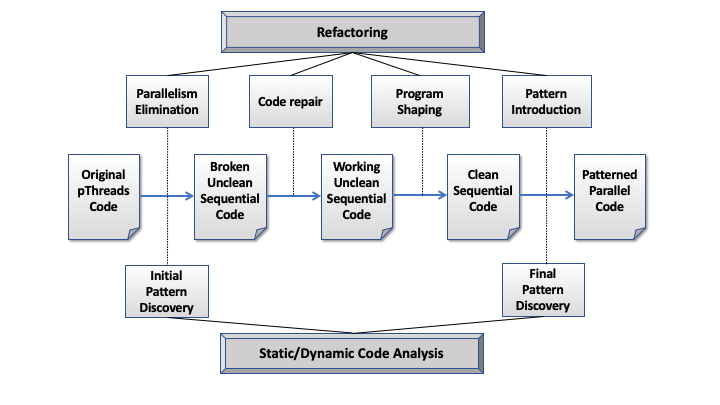
\includegraphics[width=0.78\textwidth]{images/HLPP2020Paper.png}
	\caption{Software Restoration Process}
	\label{fig:SoftRest}
\end{figure*}

%\textcolor{red}{cb: not sure we need the subseciton in the background if we have this section, or we can maybe omit or drastically cut this section down}

\noindent
In this section, we propose a new \emph{Software Restoration} methodology %based on software refactoring and code analysis
for improving the structure of legacy-parallel C++ code by applying a series of incremental program analysis and transformation steps to rewrite the code into its patterned equivalent. %In this way, w
Software restoration is based on program transformation and code analysis and aims to:
\begin{enumerate}
\item \emph{discover} the instances of common patterns in legacy-parallel code;
\item \emph{eliminate} \emph{undesirable} legacy parallel primitives from the same code; and
\item \emph{replace} the removed parallel primitives with instances of parallel patterns.
\end{enumerate}
\noindent
The input to the Software Restoration process is legacy-parallel C/C++ code that is based on some low-level parallelism library, such as pthreads, and the output is the semantically-equivalent code based on parallel patterns. In this way, we obtain well-structured code based on a higher level of parallel abstraction, which is significantly more maintainable and adaptive while still preserving
good performance of the original, highly-tuned parallel version. In this paper, we will focus on the TBB library as our target code. 

The Software Restoration methodology consists of a number of steps, each applying a class of code transformations, some of which are driven by the pattern discovery code analysis.  The whole process is depicted in Figure~\ref{fig:SoftRest}. In the below description, we will focus on the code transformation steps. We will use a synthetic, but representative, parallel pipeline as a running example in order to demonstrate the transformation. Listing~\ref{lst:simplePipe} presents aspects of the original parallel code with pthreads that are pertinent to this demonstration.

%\begin{figure}
\begin{lstlisting}[caption=Original Simple Pipeline Code,frame=single,label=lst:simplePipe]
int main(int argc, char *argv[]) {
  ...  
  // create the workers, then wait for them to finish
  pthread_create(&workerid[0], &attr, Stage1, (void *)&stage_queues[0]);
  pthread_create(&workerid[1], &attr, Stage2, (void *)&stage_queues[1]);
  pthread_create(&workerid[2], &attr, Stage3, (void *)&stage_queues[2]);
  
  for (i = 0; i < NRSTAGES; i++)
    pthread_join(workerid[i], NULL);
  
  ...
}

// Second stage reads an element from the input queue, adds 1 to it,
// and writes it to the output queue.
void *Stage2(void *arg) {
  int my_input, my_output;
  pipeline_stage_queues_t *myQueues = (pipeline_stage_queues_t *)arg;
  queue_t *myOutputQueue = myQueues->outputQueue;
  queue_t *myInputQueue = myQueues->inputQueue;

  for (my_input = read_from_queue(myInputQueue);
       my_input>0 || my_input == EOS;
       my_input = read_from_queue(myInputQueue)) {
    if (my_input != EOS) {
      my_output = my_input + 1;
      add_to_queue(myOutputQueue, my_output);
    } else { // EOS is a terminating token. Pass on if received.
      add_to_queue(myOutputQueue, EOS);
      break;
    }
  }
  return NULL;
}

void add_to_queue(queue_t *queue, int elem)
{
  pthread_mutex_lock(&queue->queue_lock);
  // If the queue is full, wait until something reads from it before adding a new element
  if (queue->nr_elements == queue->capacity)
    pthread_cond_wait(&queue->queue_cond_read,&queue->queue_lock);
  queue->elements[queue->addTo] = elem;
  queue->addTo = (queue->addTo + 1) % queue->capacity;
  queue->nr_elements++;
  pthread_cond_signal(&queue->queue_cond_write);
  pthread_mutex_unlock(&queue->queue_lock);
}
\end{lstlisting}

\noindent
In the above \lstinline|main| function (Lines 1--12), a pipeline of three stages is created using three threads. The stages are connected by queues such that all stages have an output queue, and stages two and three have an input queue. After creation, the \lstinline|main| function waits for the threads to finish their work (Lines 8--9) before continuing. In Lines 14--34, we show the function for the middle stage of the pipeline, which reads an integer from the input queue, increments it by one, then puts it into the output queue. The first and third stages have a similar structure, where the first stage acts as a source of integers for the second stage, and the third stage doubles its inputs before adding them to the final output queue.

All the relevant synchronisation code for the queues can be found in two functions: \lstinline{add_to_queue} and \lstinline{read_from_queue}. Only \lstinline{add_to_queue} (Lines 36--37) is shown here; \lstinline{read_from_queue} is similar. Both functions use one mutex lock and two conditional variables. The latter are used for synchronisation when threads are waiting to insert an element into a full queue or for reading from an empty queue (e.g.\ at the start of the program). When a thread needs to add to the queue, it first acquires the queue lock and checks if the queue is full (Lines 38--41).
%in which case writing a new element is impossible. 
When the queue is full, the thread releases the lock and waits for a signal that some other thread has consumed an element of this queue (\lstinline{queue->queue_cond_read} conditional variable, line 41). After this conditional variable is signalled, the thread enqueues the element, updating the queue counter and pointer in the process (Lines 42--44). Finally, the thread signals that an element has been added to the queue (\lstinline{queue->queue_cond_write} conditional variable, Line 45) and releases the queue lock (Line 46) before returning.

\paragraph{Parallelism Elimination.}
The initial step, \emph{Initial Pattern Discovery}, analyses the original pthreaded code and discovers those parts of it, if any, that correspond to instances of parallel patterns. In our example, this stage identifies the linear pipeline created in Lines 4--6, with the pipeline stages being the functions: \lstinline{Stage1}, \lstinline{Stage2}, and \lstinline{Stage3}. 
Following pattern discovery, the first code transformation step is applied, where pthread operations and primitives are either removed or transformed, eliminating parallelism.
%This includes the calls to \emph{pthreads} functions for thread creation, synchronisation, mutex management and so on.
In Listing~\ref{lst:simplePipe}, this impacts \lstinline|main| and \lstinline|add_to_queue|; where Listing~\ref{lst:pipeParRem} shows the resulting code.

\begin{lstlisting}[caption=Simple Pipeline Code with Parallelism Removed, frame=single, label=lst:pipeParRem]
int main(int argc, char *argv[]) {
  ...
  // Calls to pthread_create are converted to function calls.
  Stage1((void *)&stage_queues[0]);
  Stage2((void *)&stage_queues[1]);
  Stage3((void *)&stage_queues[2]);
  
  // The loop containing pthread_join is removed.
  ...
}

void add_to_queue(queue_t *queue, int elem) {
  // All mutex and conditional variable operations are removed.
  queue->elements[queue->addTo] = elem;
  queue->addTo = (queue->addTo + 1) % queue->capacity;
  queue->nr_elements++;
}
\end{lstlisting}

\noindent
%Note that all the \lstinline{pthread_} calls from the Listing~\ref{lst:simplePipe} have either been removed or replaced with the calls to the underlying functions (in the case of \lstinline{pthread_create}).
%Note, however that the code obtained in this
%way would not work.
%
%Whilst all pthread operations have been removed or transformed, and the program is now sequential, t
%
We note that the Parallelism Elimination stage \emph{does not guarantee that a program's semantics are preserved} and thus errors may be introduced.
%
%Accordingly, as in our running example, errors may be introduced.
%
Here, \lstinline|Stage1| contains a \lstinline|for|-loop that enqueues elements in its output queue. Since the second stage, which reads from that queue, is no longer consuming those elements concurrently, and the queue is smaller than the total number of elements produced, the second stage will now consume and process only a subset of its inputs in the original pthreaded version after \lstinline|Stage1| returns.
%
%Note that if the number of integers produced by \lstinline|Stage1| were infinite, or \lstinline|add_to_queue| was not implemented such that elements are overwritten when adding elements to a full queue, the loop in \lstinline|Stage1| could either loop infinitely or crash the program. 
%
%Ultimately, the semantics of the program produced by the Parallelism Elimination stage is not the same as the original pthreaded program; the code must therefore be \emph{repaired}.
%
Because the semantics of the program have changed following Parallelism Elimination, the code must be \emph{repaired}.


%function would be executed, which would just write all its outputs into its output queue (in a circular way), therefore overwriting the data possibly multiple times. After \lstinline{Stage1} finishes,
%\lstinline{Stage2} would start, read all the elements currently in its input queue (which would be just a subset of all the data produced by \lstinline{Stage1}) and write them to the output queue. It is clear that in this way there would be loss of data, so the output that the final stage produces would not be the same as in the parallel version.

\paragraph{Code Repair.}
%As observed in the previous step, Parallelism Elimination might result in code that is broken and, hence, not semantically equivalent to the original legacy-parallel code.
%
Our example is just one of many in which merely removing pthread constructs introduces errors (see Section~\ref{sec:evaluation} for more examples). The next step in Software Restoration is, therefore, to repair the potentially broken code produced by Parallelism Elimination. In general, due to the potential complexity of this repair stage, multiple transformations may need to be applied.
%
%In our pipeline example, this is actually the most complicated step of the whole methodology and the resulting code is given in Listing~\ref{lst:pipeRepaired}.

In order to effect repairs in our running example it is necessary to stop the first stage from overflowing its output queue. This can be achieved by merging the loops found in \lstinline|Stage1|, \lstinline|Stage2|, and \lstinline|Stage3|, thereby resulting in loop where the operations in stages two and three are applied to each integer produced by stage one in the same iteration that produces it. Listing~\ref{lst:pipeRepaired} represents the result of this process, where \lstinline|Stage1|, \lstinline|Stage2|, and \lstinline|Stage3| are first \emph{lifted} into a new function, \lstinline|Pipe|, and subsequently \emph{unfolded}. The \lstinline|for|-loops exposed by this unfolding are then merged, allowing all three stages to be executed within a single iteration. This avoids the first stage overflowing its output queue, and consequently, results in a program that is sequential but semantically equivalent to the original pthreaded program.

%it is necessary to immediately apply the second and third stages of the pipeline to each integer produced by the first stage.

\begin{lstlisting}[caption=Simple Pipeline Code after Code Repair, frame=single, label=lst:pipeRepaired]
void Pipe(void** a0, void* a1, void* a2, void* a3) {
  int my_output1, i1;
  pipeline_stage_queues_t *myQueues1 = (pipeline_stage_queues_t *)a1;
  queue_t *myOutputQueue1 = myQueues1->outputQueue;
  ...
  for (i1 = MAXDATA ; i1>=0; i1--) {
    if (i1 > 0) { ...
      my_output1 = i1;
    } else {
      my_output1 = EOS;
    }
    add_to_queue(myOutputQueue1, my_output1);

    my_input2 = read_from_queue(myInputQueue2);
    if (my_input2 != EOS) {
      my_output2 = my_input2 + 1;
      add_to_queue(myOutputQueue2, my_output2);
    } else {
      add_to_queue(myOutputQueue2, EOS);
    }

    my_input3 = read_from_queue(myInputQueue3);
    if (my_input3 != EOS) {
      my_output3 = my_input3 * 2;
      add_to_queue(myOutputQueue3, my_output3);
    }
  }
}
\end{lstlisting}

%\noindent 
%Here, the calls to \lstinline|Stage1|, \lstinline|Stage2|, and \lstinline|Stage3| in \lstinline|main| are first \emph{lifted} into a new function, \lstinline|Pipe|. Each of those calls are then \emph{unfolded} in order to expose the \lstinline|for|-loops that they contain. These loops are then \emph{merged}, allowing all three stages to be executed within a single iteration. This avoids the first stage overflowing its output queue, and consequently, results in a program that is sequential but semantically equivalent to the original pthreaded program.

%In order to preserve the 

%the new bounding condition (line 30) is a disjunction of the original loop bounding conditions, and the bodies of those loops are wrapped in \lstinline|if|-statements (lines 15, 19--25, 29) whose conditions are again derived from the original loop bounding conditions. This ensures that the merged loop replicates all iterations from the original separate loops, whilst at the same time ensuring that only the relevant code activates at the right time. \textcolor{red}{ab: urgh, this is horrible redo this.}

%In the listing, we show the \lstinline{main} and \lstinline{Stage2} function. Note that in the main function, the three stages of the pipeline are interleaved in the while loop (lines 4--9). The \lstinline{Stage2} function is transformed so that it performs just one iteration, with the loop in the function being eliminated. The terminating condition has been lifted from the
%\lstinline{Stage1} function into the newly introduced loop at line 4. Therefore, in the newly introduced loop, \lstinline{Stage1} generates one element and puts it into its output queue, \lstinline{Stage2} consumes the element from this output queue, processes it and puts its output in its own output queue and then \lstinline{Stage3} consumes the element from this queue, processes it and puts its output into the final queue. This is repeated until \lstinline{Stage1} generates the terminating element (\lstinline{0} in this case).

\paragraph{Program Shaping.}
%Despite correcting those errors introduced during Parallelism Removal, t
The code produced by the Code Repair stage may still contain artefacts from the original legacy parallelisation. In our running example, this includes the EOS token and intermediate queues.
%
In other examples, custom-built representations of flat data structures, e.g.\ arrays, introduced for chunking purposes may also be present.
%
These artefacts are redundant and could hinder alternative (and possibly better) parallelisations of the code. The next step is, therefore, to eliminate residual artefacts of legacy parallelism, and to improve structure where such improvements make the code more amenable to the introduction of patterned parallelism.
%
As in Code Repair, due to the potential complexity of this task, multiple transformations may need to be applied.
%
Each Program Shaping refactoring results in a program that is semantically equivalent to the one it transforms.
%
The result of the Program Shaping stage on our running example can be found in Listing~\ref{lst:pipeClean}, where both the EOS token and intermediate queues have been removed (see Section~\ref{sec:refac:shaping} for details) and the individual stages lifted back into functions.

%After the code repair step, the resulting code will be working sequential C/C++ code that can be compiled, and which can be transformed into the patterned parallel version. However, some artefacts of the legacy parallelisation may still remain in the code. In our example, these are the queues between stages of the pipeline computation, but in other examples it can also be custom-build representations of flat data structures, such as arrays. These artefacts are redundant and might actually hinder alternative (and possibly better) parallelisations of the code. The next step is, therefore, to eliminate them and restore the code in as clean state as it is possible. For our example, the resulting code (\lstinline{main} and \lstinline{Stage2} functions) are given in Listing~\ref{lst:pipeClean}.

\begin{lstlisting}[caption=Clean Sequential Simple Pipeline Code, frame=single, label=lst:pipeClean]
int S1(int i1) { ... }

int S2(int my_output1) { ... }

void S3(int my_output2, queue_t* myOutputQueue3) { ... }

void Pipe(void** a0, void* a1, void* a2, void* a3) {
  int my_output1, i1;
  ...
  for (i1 = MAXDATA ; i1 > 0; i1--) {
    S3(S2(S1(i1)), myOutputQueue3);
  }
}
\end{lstlisting}

%\noindent


%Here, calls to \lstinline|add_to_queue| and \lstinline|read_from_queue| are first \emph{unfolded}, allowing the specific read and write statements that represent the passing of data between stages to be matched and ultimately simplified to a single assignment statement between stages. The stages are then \emph{lifted} into the functions \lstinline|S1| (Line 11), \lstinline|S2| (Lines 13--19), and \lstinline|S3| (Line 21), and a \lstinline|struct| (Lines 1--9) generated to ensure that each stage is a single-input single-output function. The function composition on Line 32 is now in a form where pattern-based parallelism can be simply introduced, perhaps again by refactoring.


%\item \emph{Feature Cleanup.}  After the application of parallelism removal transformations, some artifacts of the legacy parallelisation may still remain in the code. These can be, for example, queues between stages of the pipeline computation or custom-build representations of flat data structures, such as arrays. These artifacts do not prevent the sequential version of application from running, but are redundant and might actually hinder alternative (and possibly better) parallelisations of the code. The next step is, therefore, to eliminate these artifacts and restore the code in the state as close to the original sequential code from which legacy parallelisation was derived as is possible. This is, again, done using refactorings. As we are focusing on the \emph{farm} and \emph{pipeline} parallelism, the transformations we do is removing the queues of the pipeline stages (for the \emph{pipeline} parallelism) and flattening of data structures (in the case of \emph{farm} parallelism). The Matrix Multiplication code after feature cleanup is given below

%% \begin{lstlisting}
%% static void *func (void* arg)
%% {
%%   data *input = (data *)arg;
%%   for (int i = input->start; i < input->end; i++) {
%% 	  multiply_row_by_matrix(a, i, b, res);
%%   }
%%   return (void *)0;
%% }


%% void threads_create() {
%%   int status;
%%   int count=0;
%%   in = (data *) malloc (sizeof(data) * tc);

%%   #pragma farm(func,tc)   
%%   for (int tid=0; tid<tc; tid++) {  
%%     in[tid].start = count;
%%     in[thread_ind].row_end = count + chunk;
%%     count += chunk;

%%     func(&in[tid]);
%%   }
%% }
%% \end{lstlisting}
%% The array \lstinline{in} in the Matrix Multiplication code represented a block view of the flat array of indices of the matrix rows, which was introduced for the purpose of chunking to increase parallelism granularity in the legacy parallelisation based on the \emph{farm} parallelism. The array of all the rows of matrix \lstinline{b} was divided in as many chuncks as there are threads (\lstinline{tc}) and a chunk of this array assigned to each thread. Since modern pattern libraries, such as \emph{OpenMP} and \emph{TBB} can do chunking implicitly and dynamically, based on e.g.~the current system load, there is no need for explicit chunking to remain in the sequential code, even if it is going to be turned into patterned code again. Therefore, we eliminate the array \lstinline{in} and change the loop on line XX to iterate over the array of matrix rows instead.  
  
%\item \emph{Additional Pattern Discovery.} Finally, once the code is restored into the state that is as close to the original sequential version as possible, further pattern discovery analysis can be made on it, as the feature cleanup transformations, and especially flattening of data structures and elimination of intermediate buffers/queues, might result in the code that has additional instances of parallel patterns that were not detected on the original, legacy-parallel code. This might enable us to parallelise the code in a different way than it was done in the original, legacy-parallel version, bringing possible benefits even in terms of performance.


\paragraph{Pattern Introduction.}
After the final pattern discovery analysis is performed and the final patterns to be introduced are identified, together with the locations in the code where this will be done, the final step is to introduce instances of parallel patterns into the now-clean sequential code.
The parts of the sequential code are replaced by calls to the functions from the high-level pattern libraries such as \emph{Intel TBB}~\cite{DBLP:reference/parallel/X11pz} or \emph{OpenMP}~\cite{10.1109/99.660313}.
%, or GrPPI~\cite{DBLP:journals/concurrency/AstorgaD0G17}.
This results in final, patterned parallel code that is semantically equivalent to the starting legacy-parallel code, but with much cleaner structure and simpler, higher-level code that allows easier maintainability, adaptivity and portability.
%\end{itemize}


\section{Pipeline Assumptions}
\label{sec:assumptions}

In this paper, we demonstrate our methodology on a subset of pipelines defined using pthreads. Whilst the refactorings described below apply only to this subset, they can be extended to facilitate a more general application of the restoration process.

We assume that a valid pipeline (i.e.\ a pipeline that can be restored using the below refactorings) is linear, that all tasks are generated by the first stage, and that no subsequent stages will create or destroy tasks. Moreover, we assume that the first stage of the pipeline will produce an end-of-stream (EOS) token, which is propagated through the pipeline, and results in a stage halting when it is received as input.
%
A valid pipeline is assumed to be set up in a single function containing a sequence (or loop) of \lstinline|pthread_create| calls. For each \lstinline|pthread_create(ti,...)| call there must be a corresponding \lstinline|pthread_join(ti,...)| call in the same function.
%
%\begin{lstlisting}
%t1 f(...) {
%  ...
%  pthread_create(t1,attr1,f1,args1);
%  ...
%  pthread_create(tn,attrn,fn,args2);
%  ...
%  pthread_join(t1,r1);
%  ...
%  pthread_join(tn,rn);
%  ...
%}
%\end{lstlisting}
%
%\noindent
We assume that each stage of a pipeline is run on a single thread. However, no assumptions are made regarding thread attributes, arguments passed to the function upon thread creation, or the second argument passed to \lstinline|pthread_join|.

Tasks are sent between stages in pipelines via intermediate queues.
%
Each stage of a pipeline is assumed to have an input queue, $q_1$, and an output queue, $q_2$, given that $q_1 \neq q_2$ and the output queue of stage $i$ is the input queue of stage $i+1$.
%
Pipeline stages may only communicate via these intermediate queues; for simplicity, we assume that (intermediate) stages do not access global variables.

Queues are assumed to be \emph{cyclic}. If the queue is full, and the implementation does not wait for an element to be read before adding a new element, it is assumed that the queue overwrites (unread) elements. We assume that queues use \lstinline|pthread_cond_wait|, \lstinline|pthread_cond_signal|, \lstinline|pthread_mutex_lock|, and \lstinline|pthread_mutex_unlock| operations only.
%
These restrictions are to ensure that, following Parallelism Elimination, the behaviour of the pipeline breaks in a consistent way. Any queue update functions should not be recursive.
%
Whilst we make no assumption on the size of queues, the interesting case is when queues are smaller than the total number of tasks passing through the pipeline.
%An example of a function that adds elements to an intermediate queue can be found on Lines 12--17 in Listing~\ref{lst:pipeParRem}.

Each stage of a valid pipeline is assumed to contain a loop that retrieves input and produces a modified version of it as output.
%
\begin{lstlisting}
void *Stage2(void *arg) {
  // SETUP
  ...
  for (input = read_from_queue(inputQueue);
       valid(i) || input == EOS;
       input = read_from_queue(inputQueue)) {
    if (input != EOS) {
      output = f(input);
      add_to_queue(outputQueue, output);
    } else {
      add_to_queue(outputQueue, EOS);
      break;
    }
  }
}
\end{lstlisting}
%
\noindent
The \lstinline|for|-loop is assumed to read input from the stage's input queue for each iteration, where the test expression is a disjunction permitting both EOS token and valid inputs (for some definition of valid). The test expression may be simplified by treating the EOS as a valid input.
%
The body of the loop is assumed to comprise an \lstinline|if|-statement that checks for the EOS token, represented here by a preprocessor macro. When the input is not the EOS token, it is modified (Line 8) and added to the output queue (Line 9).
%
Conversely, when the input is the EOS token, it is propagated to the next stage (Line 11) and a \lstinline|break| statement used in order to halt the stage (Line 12). Should the EOS token be handled incorrectly and not halt the stage, due to our assumptions on the nature of the intermediate queues, the \lstinline|for|-loop will wait indefinitely for input that will never arrive. Whilst we permit the occurrence of \lstinline|break| statements only in the locations specified above, we assume that no part of the pipeline has \lstinline|continue| or \lstinline|goto| statements.

The first stage differs in that the input is not retrieved from an input queue, but tasks are generated in a \lstinline|for|-loop. For example, in \lstinline|Stage1|,
%
\begin{lstlisting}
void *Stage1(void *arg) {
  t1 inputs[NINPUTS];
  ...
  for (i = 0; i<=NINPUTS; i++) {
    if (i < NINPUTS) {
      output = inputs[i];
    } else {
      output = EOS;
    }
    add_to_queue(outputQueue, output);
  }
}
\end{lstlisting}
%
an array of inputs is iterated over and each element is sent to the second stage of the pipeline.
%
We assume that the \lstinline|for|-loop in the first stage is finite and that termination is controlled by the test expression and not through a conditional statement in the body of the loop.
%
Once all tasks have been generated, the first stage will emit an EOS token and no further iterations of the loop occur.


%\begin{itemize}
%\item Linear pipelines only.
%\item We will assume the loop in the first stage of the pipeline has a finite (and obvious) bound. In examples where this does not hold (e.g.\ CB's example) we first transform infinite loops to conform.
%\item The first stage of the pipeline will produce an EOS token, and all other stages will stop (via break statement) when that EOS token is received as input.
%\item All tasks are generated by the first stage and no other stages will create or destroy tasks.
%\item Sequence of pthread creates and pthread joins, as before.
%\item Need to update the Stage definition. Describe how break and continue statements are transformed.
%\item Intermediate queues as before.
%\end{itemize}
%
%
%\noindent
%\hrulefill
%
%We consider implicit pipelines where setup consists of a sequence (or loop) of \lstinline|pthread_create| calls. For each \lstinline|pthread_create(ti,...)| call there must be a corresponding \lstinline|pthread_join(ti,...)| call in the same function.
%%
%\begin{lstlisting}
%t1 f(...) {
%  ...
%  pthread_create(t1,attr1,f1,args1);
%  ...
%  pthread_create(tn,attrn,fn,args2);
%  ...
%  pthread_join(t1,r1);
%  ...
%  pthread_join(tn,rn);
%  ...
%}
%\end{lstlisting}
%%
%\noindent
%We assume that each stage of a pipeline is run on a single thread. We make no assumptions about thread attributes, arguments passed to the function upon thread creation, or the second argument passed to \lstinline|pthread_join|.
%
%Each stage of a pipeline is assumed to have an input queue, $q_1$, and an output queue, $q_2$, given that $q_1 \neq q_2$ and the output queue of stage $i$ is the input queue of stage $i+1$. Pipeline stages may only communicate via these intermediate queues. Queues are assumed to be \emph{cyclic}, where if the queue is full but elements continue to be added, the queue overwrites (unread) elements in the queue. We assume that queues use \lstinline|pthread_cond_wait|, \lstinline|pthread_cond_signal|, \lstinline|pthread_mutex_lock|, and \lstinline|pthread_mutex_unlock| operations only. These restrictions are to ensure that, following Parallelism Elimination, the behaviour of the pipeline breaks in a consistent way. Any queue update functions should not be recursive. Whilst we make no assumption on the size of queues, the interesting case is when the output queue is smaller than the total number of elements a stage produces. An example of a function that adds elements to an intermediate queue can be found on Lines 12--17 in Listing~\ref{lst:pipeParRem}.
%
%In addition to intermediate queues, each stage of the pipeline is assumed to contain a loop.
%%
%\begin{lstlisting}
%void *Stagei(void *arg) {
%  // setup
%  ...
%
%  for (i; ...; i++) {
%    //read from input queue
%    input = read_from_queue(inputQueue);
%    //do work
%    output = f(input);
%    //push to output queue
%    add_to_queue(outputQueue, output);
%  }
%  return e;
%}
%\end{lstlisting}
%%
%\noindent
%The body of the stage loop has three stages: \emph{i)} read from the input queue, \emph{ii)} do work on the input, and \emph{iii)} write any output to the output queue. For the purpose of illustration, we assume that the stages do not contain \lstinline|break|, \lstinline|continue|, or \lstinline|goto| statements, and they may not use any global variables. We will assume that queues are accessed via local variables in each stage.

%\noindent
%\hrulefill
%
%We consider implicit pipelines that have the form:
%
%\begin{itemize}
%\item Within the same function (necessary?) there is a sequence of \lstinline|pthread_create| calls that spawn each of the stages of the pipeline. Following those \lstinline|pthread_create| calls (perhaps not \emph{immediately} following) there will be a sequence of \lstinline|pthread_join| calls.
%\item Both \lstinline|pthread_create| and \lstinline|pthread_join| calls may be in a for loop, if desired.
%\item A pipeline of $n$ stages will have $n$ threads, functions that represent the stages (get to those later). The thread attributes can be the same or differ, it does not matter. Arguments, we imagine, will be different, but I suppose do not strictly speaking need to be.
%\item For each \lstinline|pthread_create(ti,...);| call, there must be a corresponding \lstinline|pthread_join(ti,...)| call. We make no restrictions on the second argument of \lstinline|pthread_join|.
%\item Where both or either creation and join calls are in a loop, we will assume that the bound of the loop is the number of stages in the pipeline. The loops will iterate over all stages of the pipeline.
%\end{itemize}
%
%\begin{lstlisting}
%t1 f(...) {
%  ...
%  pthread_create(t1,attr1,f1,args1);
%  ...
%  pthread_create(tn,attrn,fn,args2);
%  ...
%  pthread_join(t1,r1);
%  ...
%  pthread_join(tn,rn);
%  ...
%}
%\end{lstlisting}
%
%\noindent
%Alternatively,
%
%\begin{lstlisting}
%t1 f(...) {
%  ...
%  for (i; i < MAX_THREADS; i++) {
%    pthread_create(ts[i],attr[i],fs[i],args[i]);
%  }
%  ...
%  for (i; i < MAX_THREADS; i++) {
%    pthread_join(ts[i],rs[i]);
%  }
%  ...
%}
%\end{lstlisting}
%
%\noindent
%Communication between pipeline stages.
%
%\begin{itemize}
%\item Pipeline stages may only communicate via intermediate queues. Each stage, $i$, has both an input queue, $q_1$, and an output queue, $q_2$, s.t.\ $q_1 \neq q_2$, and the input queue of stage $i+1$ is $q_2$.
%\item We assume that queues have functions to add elements to a given queue and, similarly, to remove elements from a given queue. (Signatures.)
%\item Intermediate queues are assumed to be cyclic in that if the queue is full and that things are added to that queue, it will overwrite unread elements in the queue rather than fail. In our example\dots
%\item For the purposes of our demonstration, we assume that queues use only \lstinline|pthread_cond_wait|, \lstinline|pthread_cond_signal|, \lstinline|pthread_mutex_lock|, and \lstinline|pthread_mutex_unlock| pthread operations. (This is extensible, \&c.)
%\item These functions may not be recursive. (It will get in the way of unfolding.)
%\item We make no assumptions on the size of the queues. (But we are generally interested when they are small because breakages happen when an output queue is smaller than the number of elements a stage produces.)
%\item Just point at the code we already have for this sort of thing; either that or lift it up here, and use the space elsewhere for something else.
%\end{itemize}
%
%The pipeline stages themselves.
%
%\begin{itemize}
%\item Each stage of the pipeline should contain a loop which effectively defines the behaviour of the stage itself. (Either for or while loops; maybe change them to for loops for ease and clarity.)
%\item The body of the loop has three general stages:
%  \begin{enumerate}
%  \item fetch work,
%  \item do work, and
%  \item push result of work.
%  \end{enumerate}
%\item We will generally assume that the stages do not contain \lstinline|break|, \lstinline|continue|, and \lstinline|goto| statements. (I imagine that both \lstinline|break| and \lstinline|continue| statements could potentially be transformed by wrapping things in if statements and what-have-you, but we'll leave them for the time being. Wouldn't even know where to start with \lstinline|goto| statements.)
%\item The statements must not use any global variables. (So that the only values that they can access are local, parameters, and those from their input queues.)
%\item The stages must not be recursive.
%\item Something about locking
%\item What about return statements when it ends? Not a problem, I don't think. But will need to double check.
%\end{itemize}
%
%\begin{lstlisting}
%void *Stagei(void *arg) {
%  // setup
%
%  for (i; ...; i++) {
%    //read from input queue
%    input = read_from_queue(inputQueue);
%    //do work
%    ...
%    //push to output queue
%    add_to_queue(outputQueue, output);
%  }
%  return e;
%}
%\end{lstlisting}

%\noindent
%\hrulefill
%
%\begin{enumerate}
%    \item Syntax
%        \begin{itemize}
%            \item Stages in the pipeline shouldn't have return, continue, etc. statements
%            \item each stage does not depend on variables bound in other stages or update free variables
%            \item Something to say about the set of pthread operations.
%            \item Communications are via mutex locks and conditional variables
%            \item The queue adding behaviour is that it's cyclic (with the conditional used to block when full in the original pthreaded code). (This means that we have a very specific 'broken' behaviour from when we remove the pthread operations.)
%            \item Each stage as a separate input and output queue s.t.\ the output queue of stage $i$ is the input queue of stage $i+1$.
%            \item Each function stage has a loop that starts with dequeueing and ends with enqueueing.
%            \item Show some form of template
%        \end{itemize}
%    \item Parallelism Elimination
%    \item Code Repair (Merge Loops)
%        \begin{itemize}
%        \item Sequence of for or while loops s.t.\ all of the loops are of the same kind. (So, no, e.g., while then for then while) (assume transformation into the same kind prior to this refactoring)
%        \item Something about weakening of while-loop conditions (change to for-loops?)
%        \item Infinite (really termination-obfuscated; look for break statements?) to finite loops.
%        \end{itemize}
%    \item Program Shaping
%        \begin{enumerate}
%            \item Remove Intermediate Queues
%                \begin{itemize}
%                    \item The read-write-update stuff seems okay
%                \end{itemize}
%            \item Merge Arguments
%                \begin{itemize}
%                    \item Name collisions ($\alpha$-renaming \&c.)
%                \end{itemize}
%        \end{enumerate}
%\end{enumerate}

\section{Restoration Transformations} \label{sec:refactoring}

%We propose a series of program transformations to facilitate the restoration of C programs that have been previously parallelised using low-level pthread parallelism techniques. 
%
The following transformations are grouped according to the stages in Section~\ref{sec:methodology} and all are apply to C programs that adhere to the assumptions in Section~\ref{sec:assumptions}.
%
In addition to the following, standard transformations may also facilitate the restoration process. For instance, the transformation to \emph{unfold} a function definition~\cite{darlington77} is used in both Code Repair and Shaping stages; e.g.\ in the former, it allows loops to be merged, and in the latter, it allows the elimination of intermediate queues. The \emph{extract method}~\cite{DBLP:books/daglib/0019908} transformation can be similarly used to lift a pipeline into a self-contained function, or to lift its individual stages (back) into separate functions.

%In this section we propose three refactorings to \emph{restore} C applications that have been previously parallelised using low-level pthread parallelism techniques. We divide our restoration refactorings into specific examples of eliminating \emph{pipeline} parallel (described in Section~\ref{sec:removepipeline}), and removing \emph{farm} parallelism (described in Section~\ref{sec:removefarm}).
%These restoration refactorings on both farm and pipelines are categorised by i) \emph{eliminating} the existing pthread concurrency by removing the calls to pthread functions, to they can be later replaced with calls to structured high-level algorithmic skeletons (described in Section~\ref{sec:removepthread}), ii) \emph{repairing} the eliminated versions of the code, which may have some bugs introduced by removing the underlying concurrency logic, and iii) \emph{shaping} the code, into order to structure it in a way that parallel patterns can be easily introduced. 
%We explain each of these refactorings one by one in the following subsections.

\subsection{Parallelism Elimination}
\label{sec:refac:elimination}

Parallelism Elimination comprises a single composite transformation that either removes or transforms pthread operations. As noted in Section~\ref{sec:methodology}, Parallelism Elimination
%, and by extension this transformation, 
does \emph{not} guarantee that the result of the transformation will be semantically equivalent to the transformed program. It is applied to the functions that are identified as part of the valid pipeline and effects the following transformations.
%
\begin{itemize}
\item Removes \lstinline|#include <pthread>| when all pthread operations within the file are found within the functions identified as part of the valid pipeline.
%\item Removes all mutex (\lstinline|pthread_mutex_*|), condition (\lstinline|pthread_cond_*|), and attribute (\lstinline|pthread_attr_*|) operations.
\item Removes all pthread operations within the pipeline functions aside from calls to both \lstinline|pthread_join| and \lstinline|pthread_create|.
\item Removes all variable declarations whose types are defined as part of the pthread library, excepting \lstinline|pthread_t|. This includes global declarations when those variables occur solely within the identified pipeline functions.
\item Declarations in the form \lstinline|pthread_t t;| are transformed into \lstinline|void* t;|. As above, in the case where such declarations are global, the variables may occur only in the pipeline functions.
\item Calls to \lstinline|pthread_create| of the form,
%
\begin{lstlisting}
pthread_create(t,a,f,x)
\end{lstlisting}
%
are transformed into the form:
%
\begin{lstlisting}
t = f(x);
\end{lstlisting}
%
\noindent
Recall that Parallelism Elimination converts the type of \lstinline|pthread_t| variables to \lstinline|void*| variables of the same name(s), and that \lstinline|pthread_create| requires that \lstinline|f| returns a value of type \lstinline|void*|.
%
\item Calls to \lstinline|pthread_join| are transformed according to whether the second argument is \lstinline|NULL|. When the second argument is \emph{not} \lstinline|NULL|, e.g.\ \lstinline|pthread_join(t,x)|, the join operation is transformed into the form \lstinline|x = t|. Otherwise, the call to \lstinline|pthread_join| is removed.
%  
\item In cases where a call to \lstinline|pthread_join| or \lstinline|pthread_create| forms the right-hand-side of an assignment statement, e.g.
%
\begin{lstlisting}
r = pthread_join(t,x);
\end{lstlisting}
%
in addition to the transformation of the pthread operation, an assignment statement is inserted where the variable being assigned, \lstinline|r|, is assigned the value of a successful call to the original pthread operation, here \lstinline|pthread_join| and \lstinline|0|. The assignments resulting from the transformation is:
%
\begin{lstlisting}
r = 0;
x = t;
\end{lstlisting}

 
\item Any \lstinline{for}-loop whose body contains no statements following the removal of a pthread operation will itself be removed.
\item Any \lstinline{if}-statement with a branch whose body contains no statements following the removal of a pthread operation will be transformed to have only the other branch, or itself removed, if no such branch exists. For instance, given the \lstinline{for}-loop from the synthetic pipeline example in Listing~\ref{lst:simplePipe},
%
\begin{lstlisting}[firstnumber=8]
for (i = 0; i < NRSTAGES; i++)
  pthread_join(workerid[i], NULL);
\end{lstlisting}
%
\noindent
since the second argument to \lstinline|pthread_join| is \lstinline|NULL|, the join operation result is itself a statement, and the body of the \lstinline{for}-loop contains no other operations, this \lstinline{for}-loop is removed.
\end{itemize}

%\noindent
%Other operations and types than those not listed should also be removed, but these haven't been seen/tested. (They need to be removed because otherwise you can't ) Maybe just instead say that all operations barring joins and creates should be removed.

\subsection{Code Repair}
\label{sec:refac:repair}

In addition to \emph{unfolding} and \emph{extract method} refactorings, the merging of loops is a key transformation of the Code Repair stage when restoring valid pipelines. 
%
%In the form of implicit pipelines we're considering in this paper,
%
Parallelism Elimination can result in one or more intermediate queues to overwrite elements before they can be read.
%
%In the case where a stage of the pipeline produces more output than the maximum capacity of the output queue, the queue will overwrite elements before they are read by the subsequent stage in the pipeline due to effects of Parallelism Elimination.
%
Merging the queues of all pipeline stages ensures that no queue overflows.
%
%In order to avoid the overheads involved with thread creation, individual stages of a pipeline may loop until a termination token or condition is met. Merging the loops across pipeline stages from which pthreads have been eliminated using the transformations in Section~\ref{sec:refac:elimination} can be necessary to avoid overflowing any buffers or queues in between pipeline stages, thus restoring the original semantic behaviour of the code.
%
Whilst we only describe the merging of \lstinline{for}-loops, a similar approach can be used to merge equivalent loop kinds.

%\paragraph{Merge \texttt{for}-loops}
%
%\begin{lstlisting}
%content...
%\end{lstlisting}

% We don't use merge for-loops at all any more?

\paragraph{Merge \lstinline{for}-loops.}

A sequence of $n$ \lstinline{for}-loops,
%%
%\begin{lstlisting}
%s1;
%do {
%  b1;
%} where c1;
%
%s2;
%do {
%  b2;
%} where c2;
%
%...
%
%sn;
%do {
%  bn;
%} where cn;
%\end{lstlisting}
%%
%\noindent
in the same compound statement can be merged such that the result is a single loop containing the bodies of the original loops in the same order that they appeared in the original sequence. Any statements that appear in between loops in the original code, must be commutative with respect to all preceding loops; i.e.\ it must be possible to swap the ordering of the statements and preceding loops without changing the behaviour of the program.

%To illustrate this transformation we use the below code, derived from the synthetic simple pipeline example in Section~\ref{sec:methodology}.
%
\begin{lstlisting}[caption=Intermediate Code Repair Stage for Simple Pipeline Example, label=lst:refac:repair:before, frame=single]
void Pipe(void* a1, void* a2, void* a3) {
  int my_output1, i1;
  ...
  for (i1 = MAXDATA ; i1>=0; i1--) {
    if (i1 > 0) {
      my_output1 = ...;
    } else {
      my_output1 = EOS;
    }
    add_to_queue(myOutputQueue1, my_output1);
  }

  int my_input2, my_output2;
  ...
  for (my_input2 = read_from_queue(myInputQueue2);
       my_input2>0 || my_input2 == EOS;
       my_input2 = read_from_queue(myInputQueue2)) {
    if (my_input2 != EOS) {
      ...
    } else {
      add_to_queue(myOutputQueue2, EOS);
    }
  }

  int my_input3, my_output3;
  ...
  for (my_input3 = read_from_queue(myInputQueue3);
       my_input3>0 || my_input3 == EOS;
       my_input3 = read_from_queue(myInputQueue3)) {
    if (my_input3 != EOS) {
      ...
    } else {
      break;
    }
  }
}
\end{lstlisting}
%
\noindent
Listing~\ref{lst:refac:repair:before} builds on the example in Listing~\ref{lst:pipeParRem}, where the calls to \lstinline|Stage1|, \lstinline|Stage2|, and \lstinline|Stage3| have been lifted into the function \lstinline|Pipe| using \emph{extract method} and then \emph{unfolded}.
%
It is possible to merge all three loops since the statements in between the loops can be safely executed prior to the first and second loops.
%
\begin{lstlisting}[caption=Following Merging of loops in Listing~\ref{lst:refac:repair:before}, label=lst:refac:repair:after, frame=single]
void Pipe(void** a0, void* a1, void* a2, void* a3) {
  int my_output1, i1;
  ...
  for (i1 = MAXDATA ; i1>=0; i1--) {
    if (i1 > 0) {
      my_output1 = ...;
    } else {
      my_output1 = EOS;
    }
    add_to_queue(myOutputQueue1, my_output1);

    my_input2 = read_from_queue(myInputQueue2);
    if (my_input2 != EOS) {
      ...
    } else {
      add_to_queue(myOutputQueue2, EOS);
    }

    my_input3 = read_from_queue(myInputQueue3);
    if (my_input3 != EOS) {
      ...
    }
  }
}

\end{lstlisting}
%
Since we assume that new tasks are only produced by the first stage and that all subsequent stages neither generate nor destroy tasks, it follows that the number of iterations for the first loop will be equal to the number of iterations for subsequent loops in the original pipeline.
%
Consequently, the initialisation statement, test expression, and iteration expression of the merged loop will be those of the first loop; here, \lstinline|i1 = MAXDATA|, \lstinline|i1>=-1|, and \lstinline|i1--|, respectively.
%
The bodies of the individual loops are included in the same order as the original loops themselves. Since the merged loop uses its initialisation statement, test expression, and iteration expression, the body of the first loop is included unchanged.
%
Bodies of subsequent loops, however, are preceded by their update statement. For example, the body of the second loop is preceded by the assignment to \lstinline|my_input2| on Line 12 in Listing~\ref{lst:refac:repair:after} which is taken from the update statement on Line 18 in Listing~\ref{lst:refac:repair:after}. This ensures that the input queue for each stage is read from only when a task has been added to that queue by the preceding stage.
%
In addition to the inclusion of the update expression, the \lstinline|break| statements from the original \lstinline|for|-loops are removed, leaving the propagation of the EOS token in all but the final stage. In the final stage of our pipeline (Lines 19--22) we remove the entire \lstinline|else| branch in Listing~\ref{lst:refac:repair:after} since it contains only the \lstinline|break| statement on Line 35 in Listing~\ref{lst:refac:repair:before}. Whilst the removal of these \lstinline|break| statements is not strictly necessary, since they will only be evaluated when the first stage emits an EOS token once all other tasks have been processed, they are removed because they are redundant now that the termination of the merged loop is controlled by the first stage of the pipeline, which will terminate after generating the EOS token.


%However, the bodies of the subsequent loops are included s.t.\ they are enclosed in an \lstinline|if|-statement and preceded by an assignment statement. The condition of a given \lstinline|if|-statement is the text expression of the respective loop. \textcolor{blue}{There's a point here about how because we assume that all tasks will flow through as an assumption it stands that the condition will not prematurely halt the pipeline, and so we don't need the }

%However, the bodies of the subsequent loops are included by wrapping them in an \lstinline|if|-statement, whose condition is taken from the termination expression of the original loop. Additionally, since we do not include the update expressions  For example, the loop over Lines 16--24 in Listing~\ref{lst:refac:repair:before} representing the second stage of the pipeline is transformed into the statements over Lines 12--19 of Listing~\ref{lst:refac:repair:after}.


%\noindent
%\hrulefill
%%
%\begin{itemize}
%\item The first stage remains the same. This is possible because we're using the initialisation statement, test expression, and update statement of the first loop for the merged loop. Since it also contains no break, continue, or goto statements by assumption, we are entirely safe here.
%\item Subsequent stages are wrapped in an if statement to ensure that they only fire when they are supposed to. (I wonder if this is actually redundant because all tasks must be dealt with so they all have the same number of iterations?) The condition for the if statement is taken from the condition for the relevant loop.
%\item You can't put the calls to read from queue in the initialisation statement because the queues will just return gibberish. Similarly, you can't use the calls in the iteration expression because it will return gibberish on the first two iterations for the third stage (in this specific example). Since you actually only need to read from the queue when you know that the previous stage has pushed something to the queue, it makes sense that you put the iteration expression of the loop before the if statement.
%\item The break statements in the subsequent stages will be simply be removed. We leave the statements that propagate the EOS token because I believe we'll be needing them later when converting\dots
%\item Actually, I'm not so sure. The problem we have here is that you need to get rid of the EOS at some point as it's not an output of the pipeline itself. For TBB, the EOS is a call to \lstinline|stop()| in the first stage of the pipeline. I wonder, then, if we could get rid of the EOS parts of the other stages and put a break in where we emit the EOS itself in the first stage? Then, we could convert the sole remaining break statement to \lstinline|stop|. The difficulty with this, however is whether the break would work when you lift the first stage into a function... Something to check, I think. Also, we should check how we're going from sequential code to TBB to make sure we're not missing something obvious. Ah, all we did between pth.8 and pth.9 was add an else onto the first if so I think we could probably just get rid of it entirely, adjusting the loop condition accordingly to get rid of the iteration with the EOS in it. Don't know what's best.
%\end{itemize}
%
%\noindent
%\hrulefill


%initializationStatement; testExpression; updateStatement

%\begin{itemize}
%\item The initial expression for the for loop doesn't matter; it's going to be the initial expression for the first loop as that is what sets everything off, and since the other `input' arguments aren't going to be initialised yet, it would be foolish to do so.
%\item Assumption here that the first loop represents a generator. It will stop looping if it stops/hangs at one point. It shouldn't hang because we've removed the pthread stuff; ah, but what if that pthread stuff is outside of the pipeline? Reading from a file will just continue returning EOF, I think, so that's not a problem. So, we make it so that the update function for the first loop will \emph{always} succeed, it will not fail (i.e. error out), and it will not wait on a resource.
%\item The idea is that the first for loop pertains to the first stage of the pipeline; that's obvious enough.
%\item Note that you \emph{cannot} put the iterators of later loops in the merged loop iterator because it will continue to loop infinitely (because there's no waiting when the loop is full/empty). You \emph{could} adjust the read operation, which we will suggest, but that should probably be an additional/separate refactoring or transformation, rather, which I don't want to go into here, because that's just inviting problems. Also, there's not much point because our end goal \emph{isn't} sequentialisation, but rather updating the parallelism so we're getting rid of the intermediate queues entirely.
%\item The first stage of the pipeline must represent a bound on the number of iterations, because otherwise the nature of the intermediate queues will continue to cycle through nonsense elements. (which is what causes the errors). So, let's say that the number of iterations of the first loop is a bound on those that follow. This is a sensible assumption because you're not going to get out more than you put in... or you could do, if your successive stages also generate input for the pipeline by, e.g., duplicating their input. I think we have to assume that for each stage barring the initial stage of the pipeline, you have one input and one output, and where the initial stage only has a single output. (All of this is per iteration.)
%\item I think this is an okay assumption because we're converting this into a fairly standard TBB pipeline. (I wonder if you can create a TBB pipeline where a stage may produce more output onto the output queue. It seems that you can't: `However, Filter objects in TBB can only take a single input and produce a single output.` Others have gotten around this using nested pipelines. See `Expressing Pipeline Parallelism Using TBB Constructs')
%\item This could be extended later to consider what happens when you have stages that are allowed to either remove inputs or add inputs to the stream. I think you'd have to assume some sort of adjustment to the intermediate queues, so that they return an empty operator and you would stop there.
%\item Alternatively, you might want to have it so that there are loops for each of the successive stages within the inner loops, but then that might cause a problem too what with overflow \&c. so you'd want to have a flat loop that you can easily deal with.
%\item We assume linear pipelines only. Intermediate queues may be of different sizes, but the number of tasks passed through the pipeline should be constant (i.e.\ each task generated by the first stage of the pipeline must travel through each stage of the pipeline and be introduced to the output queue).
%\end{itemize}


%
%The bounding condition of the merged loop is formed of the disjunction of the conditions of the original loops. Similarly, the body of the merged loop comprises the bodies of the original loops wrapped in \lstinline{if}-statements. The condition of one of these \lstinline{if}-statements is the \emph{weakened} condition of the respective original \lstinline{do}-loop; e.g.\ the condition \lstinline|my_input_2>0| above is weakened to \lstinline|my_input_2>=0|. This weakening is necessary, since the body of a \lstinline{do}-loop is executed before the bounding condition is checked.
%%
%% Someone is going to ask about weakening rules and how is 'weakening' defined for all the things. Annoying.
%%
%Moreover, because the loop body is guaranteed to execute once, it is possible that a variable used in the bounding condition may be declared outside of the loop, but only initialised within it. For example, in the second and third stages above, neither \lstinline|my_input_2| nor \lstinline|my_input_3| are initialised before the assignment \emph{inside} the body of their respective loops (Lines 15 \& 23, Listing~\ref{lst:refac:repair:before}). In order to merge these loops such that the second and third stages will execute, we move the aforementioned assignment statements outside of the introduced \lstinline{if}-statement around the loop body (Lines 12 \& 18, Listing~\ref{lst:refac:repair:after}). Such assignment statements can only be lifted out of the body if they themselves depend upon variables already assigned outside of the loop.
%%
%% 'assignment statements can only be lifted out of the body if they themselves depend upon variables already assigned outside of the loop' is to stop us from lifting too much of the code out of the if-statement; you only want the bare minimum.
%%
%% Question: what happens when you move something outside of the body of the if statement and the loop still allows you to run that bit of code when it wouldn't normally (according to that loop bound). Maybe it would've been better to simply convert these to for-loops after all...
%%
%% Converting a do-loop to a for loop might be the better approach.
%%
%Variables are renamed in the bodies of the loops as necessary.
%%
%%\textcolor{blue}{What if one variable (e.g.\ some iterator \lstinline|i|) is reused between loops? Note that any (re)declarations of variables (between stages) would have been dealt with at the unfolding step.}

% Note to self: seeing as this changes the behaviour of the program; how would you even account for all the possible side-conditions (formally)? You'd need to define the desired behaviour that you'd end up with. You'd probably need to be very restrictive here because otherwise you could end up allowing lots of weird behaviours; the goal of this is to make the behaviour more sensible, so... yes, you could define your transformation to do anything you desired but that doesn't necessarily a useful transformation make.

% Note to self: whilst Parallelism Elimination and Code Repair are transformations individually, together they should form a refactoring.


% I am concerned that we're spreading ourselves too generally. I fell like we should have constrained ourselves to pipelines and farms that conform to specific requirements/assumptions. Then we could always say that the requirements/assumptions can be weakened accordingly.


%\textcolor{red}{Note that we really need to eliminate the EOS token prior to removing the intermediate queues. The problem arises because we need to pair \lstinline{add_to_queue} operations with \lstinline|read_from_queue| operations and that only works at present because we've only \emph{one} of each at the end and beginning of each unfurled stage. It should really be separate from Merge Loops.}


\subsection{Program Shaping.}
\label{sec:refac:shaping}

Program Shaping represents the broadest stage in the process and presents the programmer with the largest range of choices in terms of transformations that may be effected. In addition to \emph{unfolding} definitions and creating new functions via \emph{extract method}, other standard transformations may be applied, e.g.\ \emph{dead-code elimination}~\cite{Kennedy:DeadCodeElimination}, in order to improve or simplify the structure of the code. In order to remove aspects of the code that represent optimisations enacted for the legacy parallelisation, both existing and novel transformations may be necessary. Novel transformations may include the unchunking of data, the removal intermediate, and now redundant, queues between stages, and a removal of the EOS token. In line with our running example, we propose transformations to remove EOS tokens and to remove intermediate queues.

%and a tupling (and potential localisation) of arguments to present transformations that introduce algebraic skeletons with a simple composition of single-parameter functions. In line with our running example, we propose transformations to remove intermediate queues, and to merge arguments.

\paragraph{Remove EOS Token from Merged Loops.}

Intuitively, we assume that Remove EOS Token from Merged Loops applies to the result of Merge Loops. Since termination of all stages is controlled solely by the merged loop, the EOS token is redundant and can be removed to that the resulting restored pipeline doesn't perform unnecessary work.
%
By our assumption, at the beginning of the \lstinline|for|-loop, there is an \lstinline|if|-statement that determines whether the iterator being generated by the first stage is genuine output or the EOS token. This \lstinline|if|-statement is replaced by the branch of the \lstinline|if|-statement that produces genuine output. Additionally, the text expression of the merged loop is replaced by the condition of the \lstinline|if|-statement being removed. This results in the merged loop executing one fewer iteration and the first stage of the (now-removed) pipeline no longer adding the EOS token to its output queue.
%
For all other stages of the pipeline, we replace each stage's \lstinline|if|-statement with their output branches, thus removing the EOS token behaviour.

\begin{lstlisting}[caption=Following application of Remove EOS Token from Merged Loops to Listing~\ref{lst:refac:repair:after}, label=lst:refac:removeEOS]
void Pipe(void** a0, void* a1, void* a2, void* a3) {
  int my_output1, i1;
  ...
  for (i1 = MAXDATA ; i1 > 0; i1--) {
    my_output1 = ...;
    add_to_queue(myOutputQueue1, my_output1);

    my_input2 = read_from_queue(myInputQueue2);
    my_output2 = ...;
    add_to_queue(myOutputQueue2, my_output2);

    my_input3 = read_from_queue(myInputQueue3);
    my_output3 = ...;
    add_to_queue(myOutputQueue3, my_output3);
  }
}
\end{lstlisting}
%
\noindent
Listing~\ref{lst:refac:removeEOS} gives the result of applying Remove EOS Token from Merged Loops to the code in Listing~\ref{lst:refac:repair:after}. Here, the original test expression of the merged loop, \lstinline|i1>=0| (Line 4 Listing~\ref{lst:refac:removeEOS}), has been replaced with the condition of the \lstinline|if|-statement from the first stage of the pipeline, \lstinline|i1>0| (Line 5, Listing~\ref{lst:refac:removeEOS}). That \lstinline|if|-statement has itself been replaced by its true branch. The \lstinline|if|-statements for the other two stages (Lines 13--17 and 20--22, Listing~\ref{lst:refac:removeEOS}) have similarly been replaced by their true branches, since their false branches handle the EOS token.
%Consequently, \lstinline|Pipe| no longer contains any \lstinline|break| statements in Listing~\ref{lst:refac:removeEOS}.

%\begin{itemize}
%\item The EOS token will be replaced with the TBB \lstinline|stop| function and having the EOS token still here will muck up Remove Intermediate Queues because we have multiple points where you add to the output queue. To solve this we remove the EOS token (after all, we don't need it now).
%\item Intuitively, we assume that we have the result of Merge Loops. So, we have a for-loop and we want to remove the EOS clause for the first stage that's embedded in the for loop.
%\item Meaning that we assume that at the start of our for loop, there is an if statement that determines whether the iterator is output or EOS token, and we remove the EOS token bit.
%\item We are being conservative here, but we will need to change the number of iterations that the merged loop does because otherwise we will end up with the final iteration being gibberish.
%\item Transformations:
%  \begin{enumerate}
%  \item Replace the test expression of the loop with the condition of the if statement.
%  \item Replace the if statement with the body of the output (i.e.\ non EOS) branch only.
%  \item For other stages of the (sequentialised) pipeline, and because we assume that each stage has an if-statement in it, we can simply replace those if statements with the non-EOS token branch.
%  \end{enumerate}
%\end{itemize}

\paragraph{Remove Intermediate Queues.}

%In a pthreaded pipeline, passing the result of a stage to the next can involve intermediary queues. Once the parallelism from the pipeline has been eliminated and the code repaired, so too can these queues be removed.
%
%Removing these queues not only simplifies the structure of the code, but facilitates the introduction of a skeleton implementation since such implementations handle their own queuing.
%

Following the application of Merge Loops the intermediate queues become redundant.
%
They can be removed by inspecting, matching, and transforming \emph{read}, \emph{write}, and \emph{update} operations pertaining to those queues.
%
In our recurring example we begin this process having removed the EOS token, and having \emph{unfolded} both \lstinline|add_to_queue| and \lstinline|read_from_queue| operations. Note that the \lstinline|add_to_queue| operation in the third stage is not unfolded since this is the output of the pipeline itself.
%
\begin{lstlisting}[frame=single]
void Pipe(void** a0, void* a1, void* a2, void* a3) {
  int my_output1, i1;
  ...
  for (i1 = MAXDATA ; i1 > 0; i1--) {
    ...
    myOutputQueue1->elements[myOutputQueue1->addTo] = my_output1;
    myOutputQueue1->addTo = (myOutputQueue1->addTo + 1) % myOutputQueue1->capacity;
    myOutputQueue1->nr_elements++;

    my_input2 = myInputQueue2->elements[myInputQueue2->readFrom];
    myInputQueue2->nr_elements--;
    myInputQueue2->readFrom = (myInputQueue2->readFrom + 1) % myInputQueue2->capacity;
    ...
    myOutputQueue2->elements[myOutputQueue2->addTo] = my_output2;
    myOutputQueue2->addTo = (myOutputQueue2->addTo + 1) % myOutputQueue2->capacity;
    myOutputQueue2->nr_elements++;

    my_input3 = myInputQueue3->elements[myInputQueue3->readFrom];
    myInputQueue3->nr_elements--;
    myInputQueue3->readFrom = (myInputQueue3->readFrom + 1) % myInputQueue3->capacity;
    ...
    add_to_queue(myOutputQueue3, my_output3);
  }
\end{lstlisting}
%
A variable is \emph{read} from when that variable occurs in a statement and that variable is not being \emph{updated}; e.g.\ \lstinline|capacity| on Line 7 above.
%
Similarly, a variable undergoes a \emph{write} when it is being assigned to and is not being \emph{updated}; e.g.\ \lstinline|elements|
%, specifically \lstinline|elements[myOutputQueue_1->addTo]|, 
in the first output queue is written to on Line 6.
%
Finally, a variable is \emph{updated} when it occurs in a statement that is both \emph{reading} from and \emph{writing} to that variable; e.g.\  \lstinline|addTo| in Line 7 above. Basic increment operators, e.g.\  \lstinline|nr_elements++| on Line 8, are similarly considered \emph{updates} due to their semantics.
%
%
In order to transform these \emph{read}, \emph{write}, and \emph{update} operations, we pair the operations in the order that they appear in the code and according to the variables they \emph{read}, \emph{write}, or \emph{update}, and transform those pairs according to their composition.
%
If two queues are semantically the same but referred to by different variables then they themselves will be considered the same during pairing; e.g.\ \lstinline|myOutputQueue1| and \lstinline|myInputQueue2| refer to the same intermediate queue, thus \lstinline|myOutputQueue1->elements| and \lstinline|myInputQueue2->elements| are similarly considered to be the same variable for pairing.
%
In the above example, two cases arise:
%
\begin{enumerate}
\item \emph{Updates} to variables that do not occur elsewhere in the code pertain to queue housekeeping operations are therefore removed.
%
In the above code, Lines 7, 8, 11, 12, 15, 16, 19, and 20 are all removed.

%\item A solitary \emph{read} is not transformed in any way since it represents a source stage.
%%
%In the above code, line 13

\item A \emph{write} followed by a \emph{read} is merged into a single assignment statement s.t.\ the RHS of the \emph{read} is replaced with the RHS of the \emph{write}, and where the original \emph{write} statement is removed.
%
For example, in the above code, the \emph{write} to \lstinline|elements| on Line 6 and the \emph{read} from \lstinline|elements| on Line 10 can be paired (due in part to the behaviour of the queue reading the element that has just been added). Since this represents passing \lstinline|my_output1| on Line 6 to \lstinline|my_input2| on Line 10, it is possible to remove Line 10 and transform Line 6 into the form \lstinline|my_input_2 = my_output_1|.
%
% Note that this implicitly expects that addTo and readFrom are themselves in sync/correspond; i.e. you're not adding something and then reading something completely different.
\end{enumerate}
%
An unpaired \emph{read} that is part of an \emph{update}, e.g.\ \lstinline|capacity| on Line 7, or a paired \emph{write}, e.g.\ \lstinline|addTo| on Line 6, is removed or otherwise transformed along with the \emph{update} or paired \emph{write} statement. Similarly, an unpaired \emph{read} that is part of a \emph{paired read} statement, e.g.\ \lstinline|readFrom| on Line 10, is also transformed according to the paired \emph{read} statement.
%
%We note that \emph{updates} are considered a barrier \dots
%
When applied, the above transformations result in the removal of the two intermediate queues.
%
\begin{lstlisting}[frame=single]
void Pipe(void** a0, void* a1, void* a2, void* a3) {
  ...
  for (i1 = MAXDATA ; i1 > 0; i1--) {
    my_output1 = ...;

    my_input2 = my_output1;
    my_output2 = ...;

    my_input3 = my_output2;
    my_output3 = ...;
    add_to_queue(myOutputQueue3, my_output3);
  }
\end{lstlisting}

% TODO: adjust stage three in all versions so that you have my_output_3 = -1; if (my_input_3 >=0) {...}; add_to_queue();

% Oh, they're going to complain so much about this due to all the hand-waving and caveats and coincidences.

%\paragraph{Merge Arguments.}
%
%During restoration, the stages of a pipeline may each be represented by a single function. Since the majority of patterned pipeline implementations expect pipeline stages to take a single argument, i.e.\ usually the result of the preceding stage, it may be necessary to tuple the parameters of each stage.
%%
%This can be done (semi-)automatically.
%%
%A \lstinline|struct| can be synthesised across each of the functions representing stages in the pipeline, with each function transformed to both return and take the synthesised \lstinline|struct| as its argument. In our running pipeline example, following the removal of the intermediate queues, we have three stages represented by the functions \lstinline|S1|, \lstinline|S2|, and \lstinline|S3|, respectively. \lstinline|S1| takes a pointer to an integer and returns an integer value; \lstinline|S2| takes and returns an integer value; and \lstinline|S3| takes an integer value and a pointer to its output queue and returns nothing.
%%
%\begin{lstlisting}[frame=single]
%int S1(int* i_1) {
%  int my_output_1;
%  if (*i_1 >= 0) {
%    my_output_1 = *i_1;
%    *i_1 = *i_1-1;
%  }
%  return my_output_1;
%}
%
%int S2(int my_output_1) {
%  ...
%  return my_output_2
%}
%
%void S3(int my_output_2, queue_t* myOutputQueue_3) {
%  ...
%}
%
%void Pipe(void* a1, void* a2, void* a3) {
%  ...
%  do {
%    my_output_1 = S1(&i_1);
%    my_output_2 = S2(my_output_1);
%    S3(my_output_2, myOutputQueue_3);
%  } while (i_1 >= 0 || my_output_1 > 0 || my_output_2 > 0);
%}
%\end{lstlisting}
%%
%\noindent
%Here, we observe that the result of the first two stages are used in the merged loop bounding condition and must therefore be propagated through the stages when converted to composition form. This is achieved by synthesising a new \lstinline|struct|, \lstinline|PipeStruct|, that contains all those variables used in the condition statement, and both the input and output to the pipeline.
%%
%\begin{lstlisting}[frame=single]
%struct PipeStruct {
%  // INPUTS
%  int* i_1;
%  // OUTPUTS
%  queue_t* myOutputQueue_3;
%  // USED IN LOOP CONDITION
%  int my_output_1;
%  int my_output_2;
%};
%
%PipeStruct S1(PipeStruct arg) {
%  ...
%  return arg;
%}
%
%PipeStruct S2(PipeStruct arg) {
%  ...
%  return arg;
%}
%
%PipeStruct S3(PipeStruct arg) {
%  ...
%  return arg;
%}
%
%void Pipe(void* a1, void* a2, void* a3) {
%  ...
%  do {
%    PipeStruct arg = PipeStruct {&i_1, myOutputQueue_3};
%    PipeStruct r = S3(S2(S1(arg)));
%    my_output_1 = r.my_output_1;
%    my_output_2 = r.my_output_2;
%  } while (i_1 >= 0 || my_output_1 > 0 || my_output_2 > 0);
%}
%\end{lstlisting}
%%
%\noindent
%Here, in order to introduce a TBB pipeline, we keep the input and output to the pipeline as pointers. The variables \lstinline|my_output_1| and \lstinline|my_output_2| are only used as part of the condition and are not outputs of the pipeline, as such they are stored by their value. In this particular example, it is possible to remove the second and third disjunctions and therefore remove \lstinline|my_output_1| and \lstinline|my_output_2| from \lstinline|PipeStruct|, and thus further simplify the pipeline, but this is left to another Shaping transformation or sequence of transformations.

%\noindent
%\hrulefill
%
%\begin{enumerate}
%\item Parallelism Elimination
%  \begin{enumerate}
%  \item Single refactoring that naively removes pthread operations
%    \begin{itemize}
%    \item Successfully removes:
%      \begin{itemize}
%      \item \lstinline|#include <pthread>|
%      \item \lstinline|pthread_mutex| (lock, unlock, init, type decl)
%      \item \lstinline|pthread_cond| (wait, signal, broadcast, init, type decl)
%      \item \lstinline|pthread_attr| (init and set scope)
%      \item \lstinline|pthread_join|, where 2nd arg.\ is \lstinline|NULL| (if it is assigned to a variable, we assign \lstinline|0| instead in lieu of success)
%      \end{itemize}
%    \item When an \lstinline|if|-statement or \lstinline|for|-loop only contains a removed pthread operation, we remove the statement itself.
%    \item \lstinline|pthread_create(t,a,f,x)| calls are replaced with an assignment statement \lstinline|t = f(x)| s.t.\ the type of \lstinline|t| is changed to \lstinline|void*|.
%    \item \lstinline|pthread_join(t,x);| statements are replaced with the assignment statement \lstinline|t = x;| s.t.\ the type of \lstinline|t| is changed to \lstinline|void*| (where it hasn't already been changed during refactoring of \lstinline|pthread_create| calls).
%    \item \lstinline|y = pthread_join(t,x);| statements are replaced with the block \lstinline|{y = 0; t = x;}| s.t.\ the type of \lstinline|t| is changed to \lstinline|void*| (where it hasn't already been changed during refactoring of \lstinline|pthread_create|).
%    \end{itemize}
%  \end{enumerate}
%\item Code Repair
%  \begin{enumerate}
%  \item Extract method/function. (Standard)
%  \item Unfold (Standard)
%  \item Merge loops
%    \begin{enumerate}
%    \item \lstinline|for|-loops.
%      \begin{itemize}
%      \item Loops must be in the same scope (at the same level).
%      \item Termination condition of the merged loop is a disjunction of the conditions from the original loops; initialisation and increment parts become a comma-separated list of commands from the original loops.
%      \item Bodies are wrapped in \lstinline|if|-statements. The \lstinline|if|-statement condition is the condition of the loop whence it came.
%      \item Rename variables in the loop as necessary to ensure uniqueness.
%      \item Should there be any statements in between the loops, they must commute with the first loop. (That is, you can move them above the first loop and the program is equivalent.)
%      \end{itemize}
%    \item \lstinline|do|-loops.
%      \begin{itemize}
%      \item Note that \lstinline|do|-loops check their bounding condition only after the body has been executed. This necessitates a slightly different approach to \lstinline|for|-loops.
%      \item Condition of the merged loop is a disjunction of the conditions from the original loops.
%      \item Bodies of the original loops are wrapped in \lstinline|if|-statements. The \lstinline|if|-statement condition is \emph{weakened} condition of the loop whence the body came. When that condition is an inequality over integers, such weakening refers to an increment or decrement according to the inequality.
%      \item If a variable in the loop bounding condition is declared but uninitialised at the point of the loop, and there is an assignment statement within (at the beginning of? not depending upon anything else within the loop?) the loop body, then that assignment is lifted outside of the introduced \lstinline|if|-statement body. (If it's uninitialised outside of the loop then that part of the merged loop will never execute.)
%      \item Rename variables in the loop as necessary to ensure uniqueness.
%      \item Should there be any statements in between the loops, they must commute with the first loop. (That is, you can move them above the first loop and the program is equivalent.)
%      \end{itemize}
%    \end{enumerate}
%  \end{enumerate}
%\item Shaping
%  \begin{itemize}
%  \item Unfold (again, standard)
%  \item Extract function/method (again, standard)
%  \item Remove Queues (matching and handling reads, writes, and updates)
%    \begin{itemize}
%    \item Assume that any queuing operations have been unfolded (so that we're dealing with basic assignment statements).
%    \item A variable is \emph{read} from when that variable occurs in a statement (on the RHS of an assignment statement) and that variable is not being \emph{updated}. For example, \lstinline|myOutputQueue_1->addTo = (myOutputQueue_1->addTo + 1) % myOutputQueue_1->capacity| is a read of \lstinline|myOutputQueue_1->capacity|.
%    \item A variable undergoes a \emph{write} when it is being assigned to and is not being \emph{updated}. For example, in  \lstinline|myOutputQueue_1->elements[myOutputQueue_1->addTo] = my_output_1|, this is a write to \lstinline|myOutputQueue_1->elements|.
%    \item A variable is \emph{updated} when it occurs in a statement that is both \emph{reading} from and \emph{writing} to it. The \lstinline|myOutputQueue_1->addTo| in the read example above is an example; so too are basic increment operators, e.g.\  \lstinline|myOutputQueue_1->nr_elements++|.
%    \item Queue operations are matched in the order they appear in the code, according to the variables they read, write, or update.
%    \begin{lstlisting}
%  ...
%  myOutputQueue_1->elements[myOutputQueue_1->addTo] = my_output_1;
%  myOutputQueue_1->addTo = (myOutputQueue_1->addTo + 1) % myOutputQueue_1->capacity;
%  myOutputQueue_1->nr_elements++;
%}
%
%int elem_2;
%elem_2 = myInputQueue_2->elements[myInputQueue_2->readFrom];
%myInputQueue_2->nr_elements--; // this would be classified as a write?
%...
%  myOutputQueue_2->elements[myOutputQueue_2->addTo] = my_output_2;
%  ...
%    \end{lstlisting}
%    
%    \noindent
%    Here, for example, the write to \lstinline|elements| in line 2 would be matched with the read in line 9. \emph{Updates} are not matched with subsequent reads, writes or updates since they are considered to be standalone; e.g.\ the update to \lstinline|nr_elements| in line 5 is \emph{not} matched with the subsequent update on line 10. Moreover, updates act as a barrier for reads and writes of that same variable; e.g.\ \lstinline|addTo| is \emph{read} on line 2, \emph{updated} on line 3, and \emph{read} on line 11, but the two reads are \emph{not matched}. Reads and reads can be otherwise matched, as can reads and writes. The order in which the read and write occurs matters.
%    \item Cases:
%      \begin{enumerate}
%      \item \emph{Updates} to variables that are not used (do not occur) elsewhere in the code \emph{are removed}. (These (should) pertain to housekeeping statements around the queues.)
%      \item An unmatched \emph{read} is left as-is (because it should be a source).
%      \item A \emph{write} followed by a \emph{read} is merged into a single assignment statement s.t.\ the RHS of the read is replaced with the RHS of the write, where the original write statement is removed. (Pertains to passing from stage to the next.)
%      \item An unmatched \emph{write} is left (because it should be a sink).
%      \end{enumerate}
%    \item This is almost certainly going to be the refactoring they complain about most.
%    \end{itemize}
%  \item Merge arguments 
%    \begin{itemize}
%    \item Synthesise a \lstinline|struct| containing all input, output, and intermediate variables; input and output variables should be pointers.
%    \item The synthesised \lstinline|struct| should include global variables (all variables should be local going through the pipeline).
%    \item Transform the formal parameters of the function(s) to be only the synthesised \lstinline|struct|, with all occurrences of the merged arguments now pointing at those contained within the \lstinline|struct|. The return type and value should be transformed to the same synthesised \lstinline|struct|.
%    \end{itemize}
%  \item Remove intermediate temporary variables. Go from
%  \begin{lstlisting}
%x1 = f1(...);
%x2 = f2(x2);
%...
%  \end{lstlisting}
%  to \lstinline|fn(...f2(f1(...))...)|
%  \item Dead-code Elimination (Standard)
%  \end{itemize}
%\end{enumerate}
%
%\noindent
%Note that when removing farms in blacksholes and mandelbrot (and Vladimir's matrix multiplication?) the data that is being farmed has been chunked. Thus you can't just remove the outer \lstinline|for|-loop before Parallelism Elimination. I imagine that once you've eliminated parallelism and fixed the code, Shaping can be used to remove this chunking; this is without the scope of this paper.
%
%\begin{lstlisting}[frame=single,numbers=left,label=lst:simplefarmexample,caption={Simple farm example, based on Matrix Multiplication}]
%static void* thread_func (void* arg) {
%  input_data *input = (input_data *)arg;
%  for (unsigned int i = input->row_start; i < input->row_end; i++) {
%    multiply_row_by_matrix(a, i, b, res);
%  }
%  return (void *)0;
%}
%
%void threads_create() {
%  pthread_attr_t attr;
%  int status;
%  ...
%  status = pthread_attr_init(&attr);
%  ... 
%  int chunk = chunk_size + extra;
%  in[thread_ind].row_start = count;
%  in[thread_ind].row_end = count + chunk;
%  count += chunk;
%  
%  for (unsigned int thread_ind = 0; thread_ind < thread_count; thread_ind++) {
%    ...
%    pthread_create(&threads[thread_ind], &attr, &thread_func, &in[thread_ind]);
%  }
%}
%
%int main (int argc, char *argv[]) {
%  ...
%  threads_create();
%  
%  for (int i=0; i<thread_count; i++)
%    pthread_join (threads[i], NULL);
%  
%  pthread_exit ( NULL );        /* Let threads finish */
%}
%\end{lstlisting}

%\iffalse
%In this section we propose three refactorings to \emph{restore} C applications that have been previously parallelised using low-level pthread parallelism techniques. We divide our restoration refactorings into specific examples of eliminating \emph{pipeline} parallel (described in Section~\ref{sec:removepipeline}), and removing \emph{farm} parallelism (described in Section~\ref{sec:removefarm}).
%These restoration refactorings on both farm and pipelines are categorised by i) \emph{eliminating} the existing pthread concurrency by removing the calls to pthread functions, to they can be later replaced with calls to structured high-level algorithmic skeletons (described in Section~\ref{sec:removepthread}), ii) \emph{repairing} the eliminated versions of the code, which may have some bugs introduced by removing the underlying concurrency logic, and iii) \emph{shaping} the code, into order to structure it in a way that parallel patterns can be easily introduced. 
%We explain each of these refactorings one by one in the following subsections.
%
%\subsection{Removing Pthread Concurrency} \label{sec:removepthread}



%\begin{enumerate}
%
%\item \textbf{Replace \lstinline|pthread_create| with a function call}
%
%This refactoring replaces a call to \lstinline|pthread_create| with a function call. Any formal arguments that were originally passed to the thread, are passed to the function instead. The return result of the function, originally captured as a variable argument to \lstinline|pthread_create| is assigned to the variable instead. For instance, the example 
%
%
%	\begin{lstlisting}[frame=single]
%	var = pthread_create(&thread, NULL, f, args);
%	\end{lstlisting}
%
%can be refactored into:
%
%
%	\begin{lstlisting}[frame=single]
%	var = 0;
%	f(args);
%	\end{lstlisting}
%
%
%Here \texttt{var} is assigned \texttt{0} in lieu of the original return value of \lstinline|pthread_create| when the call is successful. The refactoring assumes that \lstinline|f| 
%%communicates with other threads via mutexes or semaphores, and 
%does not itself return a non-null value \emph{via} \lstinline|pthread_exit|. The refactoring can therefore only be applied when the body of \lstinline|f| contains only calls to \lstinline|pthread_exit| to which \lstinline|NULL| is passed as its argument. % \forall pthread_exit(var) \in f.statements.transclosure, var = NULL
%If the \lstinline{pthread_create} is within some arbitrary nesting of statements or expressions, then the same refactoring can still be applied, by first lifting (and therefore introducing an assignment of) the \lstinline{pthread_create} call first, therefore arriving at the refactored example above.
%
%\item \textbf{Replace \lstinline|pthread_exit| with a return statement}
%
%This refactoring replaces a call to \lstinline|pthread_exit| with a return statement. The argument originally passed to \lstinline|pthread_exit| are instead passed to the return statement. Consider the following example.
%
%\begin{lstlisting}[frame=single]
%pthread_exit(var);
%\end{lstlisting}
%
%\noindent
%is refactored into
%
%\begin{lstlisting}[frame=single]
%return var;
%\end{lstlisting}
%
%\noindent
%where \lstinline|var| may either be a variable or \lstinline|NULL|. Unlike the refactorings that replace \lstinline|pthread_create| and \lstinline|pthread_join|, this refactoring does \emph{not} require \lstinline|var| to be \lstinline|NULL| since both cases can be refactored in the same way. Although trivial, this is an important transformation step to removing concurrency that forms our complete methodology.
%
%
%%Whilst this refactoring allows for spawned functions to return values \emph{via} \lstinline|pthread_exit| and \lstinline|pthread_join|, the other refactorings defined and used herein assume that only functions that 
%
%%\noindent
%%\emph{Note that if \lstinline|var| \emph{isn't} \lstinline|NULL| then the result of the refactored \lstinline|pthread_create| needs to be captured. (Where? At the point of \lstinline|pthread_join|? At the point of \lstinline|pthread_create|?) Assume it only returns \lstinline|NULL| for consistency?}
%
%\item \textbf{Remove \lstinline|pthread_join|}
%
%This refactoring removes a call to \lstinline|pthread_join| when its second argument is \lstinline|NULL|; i.e.\ when it does \emph{not} expect a value to be returned from the exiting thread. As with \lstinline|pthread_create|, when the result of a call to \lstinline|pthread_join| is assigned to a variable, e.g.\
%
%\begin{lstlisting}[frame=single]
%var = pthread_join(thread, NULL);
%\end{lstlisting}
%
%\noindent
%the statement is refactored into the assignment:
%
%\begin{lstlisting}[frame=single]
%var = 0;
%\end{lstlisting}
%
%\noindent
%where \lstinline|0| is again the value returned by \lstinline|pthread_join| when it is successful. 
%
%%\emph{Again, what happens when it's part of another statement (e.g.\ if-statement) or another expression? Lift into a variable and replace call sites with that variable. In which cases does the change in order of expressions affect the external behaviour?}
%
%\end{enumerate}
%
%%\subsection{Farm Removal}
%%
%%\begin{itemize}
%%\item Matrix Multiplication example
%%  \begin{itemize}
%%  \item \texttt{discovery-examples/matmult/matmult\_pthreads.cpp}
%%  \end{itemize}
%%\item Points of note
%%  \begin{itemize}
%%  \item Global
%%    \begin{itemize}
%%    \item \lstinline|#include <pthread.h>|
%%    \item \lstinline|pthread_t *threads| (remove assignment in \lstinline|threads_create|)
%%    \end{itemize}
%%  \item \lstinline|main|
%%    \begin{itemize}
%%    \item \lstinline|pthread_join(NULL)|
%%    \item \lstinline|pthread_exit(NULL)| (transform to: \lstinline|return(NULL)|)
%%    \end{itemize}
%%  \item \lstinline|threads_create|
%%    \begin{itemize}
%%    \item \lstinline|pthread_attr_t attr| (remove \lstinline|pthread_attr_init|, replace with \lstinline|status = 0| to satisfy the if-statement at line 105)
%%    \item \lstinline|pthread_create| (rewrite to \lstinline|status=0;thread_func(threads[thread_ind])|)
%%    \end{itemize}
%%  \end{itemize}
%%\end{itemize}
%
%\subsection{Pipeline Parallelism Removal} \label{sec:removepipeline}
%
%\begin{lstlisting}[frame=single,numbers=left,label=lst:simplepipeexample,caption={Simple pipeline example, based on PGPry, from the Parsec benchmark suite.}]
%..
%pthread_t one, two;
%int shared = 0;
%pthread_mutex_t mut;
%void *StageOne(void *threadarg1) {
%  for (int i1 = 0; i1 < 5; i1++) {
%    pthread_mutex_lock(&mut);
%    int loc_shared = shared;      // Read shared
%    pthread_mutex_unlock(&mut);
%    ...
%    pthread_mutex_lock(&mut);
%    shared = loc_shared++;     // Update shared
%    pthread_mutex_unlock(&mut);
%    }
%  pthread_exit(NULL);
%}
%void *StageTwo(void *threadarg2) {
%  for (int i2 = 0; i2 < 5; i2++) { 
%    pthread_mutex_lock(&mut);
%    int loc_shared = shared;     // Read shared
%    pthread_mutex_unlock(&mut);
%    ...
%    pthread_mutex_lock(&mut);
%    shared = loc_shared--;      // Update shared
%    pthread_mutex_unlock(&mut);
%    }
%  pthread_exit(NULL);
%}
%... main () {
%  int status;
%  status = pthread_create(&one, NULL, StageOne, NULL);   // Stage One
%  if (status != 0) exit(-1);
%  status = pthread_create(&two, NULL, StageTwo, NULL);  // Stage Two
%  if (status != 0) exit(-1);
%  pthread_join(one, NULL);
%  pthread_join(two, NULL);
%}
%\end{lstlisting}
%
%%\paragraph]{Very Simple Example.}
%
%%Simplified PGPry example (Listing~\ref{lst:simplepipeexample}). A two-stage pipeline with farms for the stages. An integer represents the (size of a) buffer between stages. Parallelism removal assumes perfect scheduling for the sequential version; practically, we do not see exactly the same behaviour for the sequential version as we do the parallel versions (for all runs of the parallel version).
%\noindent
%Instances of the \emph{pipeline} pattern (see Section~\ref{sec:background}) occur frequently in legacy code involving pthreads. Typically, these instances incur two or more stages that interact with each other in an implicit way. For example, through the update of a shared variable between threads. For example, Listing~\ref{lst:simplepipeexample} shows a two-stage pipeline example, where each stage is also a \emph{farm}. This example is a simplified version of the PGPry example, taken from the Parsec Benchmark Suite~\cite{10.1145/1454115.1454128}. In the example, an integer is used to represent the size of a buffer between stages (\lstinline|i1| at Line 6, and \lstinline|i2| at Line 18).
%These stages are:
%
%\textbf{Stage 1} removes the direct calls to the pthread API, (as described in Section~\ref{sec:removepthread}). For example, this includes in \lstinline|main|, replacing \lstinline|pthread_create| calls with an assignment to \lstinline|status| and a call to the spawned function. This ensures that \lstinline|status| is initialised for the subsequent uses of it; and that values assigned should be the default successful returned value of \lstinline|pthread_create|.
%\begin{lstlisting}[frame=single]
%// status = pthread_create(&one, NULL, StageOne, NULL);
%status = 0;
%StageOne(0);
%if (status != 0) {
%  exit(-1);
%}
%\end{lstlisting}
%\noindent
%This stage also considers the \lstinline|pthread_join| calls in \lstinline|main|. Since these do not expect return values (i.e.\ their second argument is \lstinline|NULL|), so they can just be removed.
%The final refactoring in this stage is to replace the \lstinline|pthread_exit| calls with \lstinline|return NULL;|
%
%\textbf{Stage 2} unifies the stages of the pipeline together, forming a single unified stage in the form of a newly introduced function, as illustrated in the code below. The free variables in the original stages are captured as arguments to the newly introduced unified stages. Bound variables are declared in the unified stage up to alpha-renaming to preserve freshness and the binding structure of the stages. 
%
%  \begin{lstlisting}[frame=single]
%// Stage One:
%int i1;
%for (i1 = 0; i1 < 5; i1++) {...}
%// Stage Two:
%int i2;
%for (i2 = 0; i2 < 5; i2++) {...}
%// Unifies to:
%int i1;
%int i2;
%for (i1 = 0, i2 = 0; i1 < 5 || i2 < 5; i1++, i2++) {...}
%\end{lstlisting}
%\noindent
%Typically, the original stages of the pipeline will contain loops; these will be unified together by forming the disjunction of the conditionals from all the loops.
% This process is done by unifying from the first stage, then the second stage, and so on. There may be duplicated portions of the code as a result of the stage. This duplicate code can be filtered out by using common \emph{clone detection} techniques, commonly found in the literature, such as [BLAH]. Any code that occurs before any \emph{read} or \emph{write} operations on any shared data can simply be inserted into the unified stage. 
% 
%\begin{lstlisting}[frame=single]
%int i1;
%int i2;
%for (i1 = 0, i2 = 0; i1 < 5 || i2 < 5; i1++, i2++) {
%  int loc_shared1 = shared;
%  sleep(1); // representing block code
%  ...
%}
%\end{lstlisting}
%\noindent
%\textbf{Stage 3} attempts to match the \emph{reads} and \emph{writes} to the shared state that occurs in the various original stages of the pipelines. These need to be unified in such a way that order of execution is preserved in the unified stage. Operations on the state can be matched accordingly. Match \emph{read} operations on the shared state with other \emph{read} and \emph{write} operations on the shared state. In the example, a \emph{read} is matched with a \emph{read}, resulting in picking the \emph{read} operation in the first stage; here, the assignment to \lstinline|loc_shared|, occurring in \lstinline|StageOne| and \lstinline|StageTwo| (Lines 8 and 20) of Listing~\ref{lst:simplepipeexample} can be merged together to form a single assignment statement (as illustrated at Line 4 in the listing below).
%\begin{lstlisting}[frame=single]
%int i1;
%int i2;
%for (i1 = 0, i2 = 0; i1 < 5 || i2 < 5; i1++, i2++) {
%   int loc_shared = shared;
%   ...
%}
%\end{lstlisting}
%
%\noindent
%A \emph{write} operation (see Section~\ref{sec:readwrite}) in the first stage is matched with another \emph{write} operation in the second (and subsequent) stages. In Listing~\ref{lst:simplepipeexample}, we see a \emph{write} to the shared variable \lstinline|loc_shared| on Line 12, in \lstinline|StageOne| and also on Line 24, in \lstinline|StageTwo|. Here, we execute the \emph{write} instruction \lstinline|loc_shared++| from \lstinline|StageOne| first, and then we execute the \emph{write} instruction, \lstinline|loc_shared--|, from \lstinline|StageTwo|. Indeed, in this example, there is an interesting observation that these two operations will functionally cancel each other out, as incrementing a variable, and then immediately decrementing it, is obviously a \emph{cancelling} behaviour; however, reasoning about the behaviour of the operations outside of a basic \emph{read/write} behaviour is beyond the scope of this paper.
%
%  \begin{lstlisting}[frame=single]
%int i1;
%int i2;
%for (i1 = 0, i2 = 0; i1 < 5 || i2 < 5; i1++, i2++) {
%  int loc_shared1 = shared;
%  sleep(1); // representing block code
%  shared = loc_shared1++;
%
%  int loc_shared2 = shared;
%  sleep(1); // representing block code
%  shared = loc_shared2--;
%}
%\end{lstlisting}
%
%\noindent
%\textbf{Stage 4} replaces the original code in the \lstinline{main} function (Lines 29 -- 36 of Listing~\ref{lst:simplepipeexample}) with a call to the new unified function (here renamed to something more meaningful).
%
%  \begin{lstlisting}[frame=single]
%int main () {
%  int status;
%  SynthesisedPipe(NULL, NULL); // StageOne and StageTwo combined.
%  if (status != 0) exit(-1);
%}
%\end{lstlisting}
%
%\noindent
%\textbf{Stage 5} the parallelisation of the sequentialised version of the code can now be performed. Here, we now take the introduced function, and derive \emph{pipeline} stages from it, so that a patterned version can be introduced, using a framework like OpenMP~\cite{10.1109/99.660313}, Intel's Threading Building Blocks~\cite{DBLP:reference/parallel/X11pz}, or GrPPI~\cite{DBLP:journals/concurrency/AstorgaD0G17}. Here, any free variables in the refactored functions/pipeline stages need to be captured. Therefore a \lstinline|struct| is declared at Lines 1 and 13, representing the return types of the pipline stages \lstinline|S1| and \lstinline|S2|. Any global variables that previously were assigned to the results of these stages are now captured; for example at Lines 31 and 35. Note here that \lstinline{S2} takes as a parameter the updated variable \lstinline{shared} at Line 33. 
%
%\begin{lstlisting}[frame=single]
%int main() {
%...
%struct pipe_result = SynthesisedPipe(NULL, NULL, shared);
%shared = pipe_result.shared;
%...
%}
%\end{lstlisting}
%The \lstinline|struct| can be automatically generated itself, where the fields are all free variables (i.e.\ the globals) in the synthesised function.
%%
%We finally parallelise the refactored code using a clean pattern method of parallelisation, such as GrPPI.
%
%\begin{lstlisting}[frame=single]
%void* SynthesisedPipe(void* threadarg1, void* threadarg2, int shared) {
%int i1;
%int i2;
%for (i1 = 0, i2 = 0; i1 < 5 || i2 < 5; i1++, i2++) {
%  #pragma grppi seq stage
%  tuple1 ret1 = S1(i1, shared);
%  i1 = ret1.i1;
%  shared = ret1.shared;
%
%  #pragma grppi seq stage
%  tuple2 ret2 = S2(i2, shared);
%  i2 = ret2.i2;
%  shared = ret2.shared;
%  }
%  return NULL;
%}
%\end{lstlisting}
%\fi

%\paragraph{Refactoring stages.}
%\iffalse
%
%
%\begin{enumerate}
%\item In \lstinline|main|, remove farms over pipeline stages by removing the for loops surrounding them.
%\begin{lstlisting}[frame=single]
%for(i = 0; i < NUM_THREADS; i++) {
%  ...
%  rc = pthread_create(&threads[i], NULL, StageOne, arg);
%  ...
%}
%\end{lstlisting}
%Farms are for loops that contain a \lstinline|pthread_create| call. What if the for loops also calculate something else? Assume that a pragma indicating a farm stage is okay for transformation. Alpha renaming of local variables declared inside the loop body where necessary. Result of the above:
%\begin{lstlisting}[frame=single]
%...
%rc1 = pthread_create(&threads[i], NULL, StageOne, arg1);
%...
%\end{lstlisting}
%\item Still in \lstinline|main|, rewrite the \lstinline|pthread_create| calls as function calls.
%\begin{lstlisting}[frame=single]
%rc = 0;
%StageOne(arg1);
%\end{lstlisting}
%As before, since the result of \lstinline|StageOne| is assigned to a \lstinline|status|-type variable, here \lstinline|rc|, we assign the default positive result of \lstinline|pthread_create| to that variable before calling the spawned function, here \lstinline|StageOne|.
%
%\end{enumerate}
%
%\fi
%%
%\begin{enumerate}
%	\item .
%%\item In \lstinline|main|, replace \lstinline|pthread_create| calls with an assignment to \lstinline|status| and a call to the spawned function. Ensures that \lstinline|status| is initialised for the subsequent uses of it; value assigned should be the default successful returned value of \lstinline|pthread_create| (here, that's \lstinline|0|).
%%\begin{lstlisting}[frame=single]
%%// status = pthread_create(&one, NULL, StageOne, NULL);
%%status = 0;
%%StageOne(0);
%%if (status != 0) {
%%  exit(-1);
%%}
%%\end{lstlisting}
%
%%\item In \lstinline|main|, consider \lstinline|pthread_join| calls. Since these do not expect return values (i.e.\ second argument is \lstinline|NULL|), they can just be removed.
%%
%%\item Replace \lstinline|pthread_exit| calls with \lstinline|return NULL;|
%
%%\item Unify stages; of interest: the for-loops. What sort of loops can we handle? Unification synthesises a new function, the body of which is the result of said unification. Arguments to this function are the concatenation of arguments to the original stage functions.
% % \begin{enumerate}
%%  \item Unification of the conditions by disjunction. \emph{Suspect that the bodies of the separate loops need to be themselves in if-statements (with original conditions); otherwise may run stage code more often than expected.}
%%  \begin{lstlisting}[frame=single]
%%  // Stage One:
%%  int i1;
%%  for (i1 = 0; i1 < 5; i1++) {...}
%%  // Stage Two:
%%  int i2;
%%  for (i2 = 0; i2 < 5; i2++) {...}
%%  // Unifies to:
%%  int i1;
%%  int i2;
%%  for (i1 = 0, i2 = 0; i1 < 5 || i2 < 5; i1++, i2++) {...}
%%  \end{lstlisting}
%  
%%  \begin{enumerate}
%%%  \item To begin with, unify from first stage. Pass through the first stage, followed by the second stage. Question of duplicating block code. Standard blocks of code before any \emph{read}/\emph{write} operation on the shared state can just be inserted.
%%
%%%  \item Operations on the state can be matched accordingly. Match \emph{read} operations on the shared state with other \emph{read} and \emph{write} operations on the shared state. In the example, a \emph{read} is matched with a \emph{read}, resulting in picking the \emph{read} operation in the first stage; here, the assignment to \lstinline|loc_shared|.
%%%  \begin{lstlisting}[frame=single]
%%%  int i1;
%%%  int i2;
%%%  for (i1 = 0, i2 = 0; i1 < 5 || i2 < 5; i1++, i2++) {
%%%    int loc_shared = shared;
%%%    ...
%%%  }
%%%  \end{lstlisting}
%%\item  Combinations (taken in order):
%%  \begin{enumerate}
%%  \item \emph{read/read}: pick stage one read
%%  \item \emph{read/write}: replace \emph{read} RHS with \emph{write} (stage two assignment)
%%  \item \emph{write/read}: replace \emph{read} RHS with \emph{write} (stage one assignment)
%%  \item \emph{write/write}: pick stage one write
%%  \end{enumerate}
%%  \emph{These need checking.} Alpha-rename as necessary.
%%  
%%%  \item Block code from the first stage is inserted since it has no impact on the shared state.
%%%  \begin{lstlisting}[frame=single]
%%%  int i1;
%%%  int i2;
%%%  for (i1 = 0, i2 = 0; i1 < 5 || i2 < 5; i1++, i2++) {
%%%    int loc_shared1 = shared;
%%%    sleep(1); // representing block code
%%%    ...
%%%  }
%%%  \end{lstlisting}
%%%  
%%%  \item A \emph{write} operation in the first stage is matched with another \emph{write} operation in the second stage. Use the \emph{write} operation from the first stage. \emph{Are we really unifying here? We seem to be just placing stage two after stage one in a new for loop\dots}
%%%  \begin{lstlisting}[frame=single]
%%%  int i1;
%%%  int i2;
%%%  for (i1 = 0, i2 = 0; i1 < 5 || i2 < 5; i1++, i2++) {
%%%    int loc_shared1 = shared;
%%%    sleep(1); // representing block code
%%%    shared = loc_shared1++;
%%%    printf("(1-%i) shared = %i\n", i1, shared);
%%%    ...
%%%  }
%%%  \end{lstlisting}
%%  
%%  \item End of \lstinline|StageOne|, start with \lstinline|StageTwo|;
%%    \begin{enumerate}
%%    \item \emph{read/read};
%%    \item block code;
%%    \item \emph{write/write};
%%    \end{enumerate}
%%  \begin{lstlisting}[frame=single]
%%  int i1;
%%  int i2;
%%  for (i1 = 0, i2 = 0; i1 < 5 || i2 < 5; i1++, i2++) {
%%    int loc_shared1 = shared;
%%    sleep(1); // representing block code
%%    shared = loc_shared1++;
%%    printf("(1-%i) shared = %i\n", i1, shared);  
%%   
%%    int loc_shared2 = shared;
%%    sleep(1); // representing block code
%%    shared = loc_shared2--;
%%    printf("(2-%i) shared = %i\n", i2, shared);
%%  }
%%  \end{lstlisting}
%%    
%%  \item \lstinline|return NULL;| statements are the same in both stages.
%%  \begin{lstlisting}[frame=single]
%%  int i1;
%%  int i2;
%%  for (i1 = 0, i2 = 0; i1 < 5 || i2 < 5; i1++, i2++) {
%%    int loc_shared1 = shared;
%%    sleep(1); // representing block code
%%    shared = loc_shared1++;
%%    printf("(1-%i) shared = %i\n", i1, shared);  
%%   
%%    int loc_shared2 = shared;
%%    sleep(1); // representing block code
%%    shared = loc_shared2--;
%%    printf("(2-%i) shared = %i\n", i2, shared);
%%  }
%%  return NULL;
%%  \end{lstlisting}
%%  
%%  \item In \lstinline|main|, the synthesised function is called in place of the last pipeline stage.
%%  \begin{lstlisting}[frame=single]
%%  int main () {
%%    int status;
%%  
%%    // Stage One
%%    status = 0;
%%    // StageOne(NULL);
%%    if (status != 0) {
%%      exit(-1);
%%    }
%%  
%%    // Stage Two
%%    status = 0;
%%    // StageTwo(NULL);
%%    SynthesisedPipe(NULL, NULL); // StageOne and StageTwo combined.
%%    if (status != 0) {
%%      exit(-1);
%%    }
%%  
%%    return 0;
%%  }
%%  \end{lstlisting}
%%  \end{enumerate}
%
%\item Make global variables local for the synthesised function. Synthesised function needs to take additional arguments that are the global variables used within the function, and needs to return a tuple, i.e.\ \lstinline|struct|, of the global variables. The returned values of the global variables are then reassigned to their respective globals.
%\begin{lstlisting}[frame=single]
%int main() {
%  ...
%  struct pipe_result = SynthesisedPipe(NULL, NULL, shared);
%  shared = pipe_result.shared;
%  ...
%}
%\end{lstlisting}
%The \lstinline|struct| can be automatically generated itself, where the fields are all free variables (i.e.\ the globals) in the synthesised function.
%
%\item Split into separate worker functions for pipeline introduction via Grppi refactorings. \emph{Were the pipeline refactorings ever published?}
%\begin{lstlisting}[frame=single]
%void* SynthesisedPipe(void* threadarg1, void* threadarg2, int shared) {
%  int i1;
%  int i2;
%  for (i1 = 0, i2 = 0; i1 < 5 || i2 < 5; i1++, i2++) {
%    // Stage One
%    int loc_shared1 = shared;
%    sleep(1); // representing block code
%    shared = loc_shared1++;
%    printf("(1-%i) shared = %i\n", i1, shared);  
%   
%    // Stage Two
%    int loc_shared2 = shared;
%    sleep(1); // representing block code
%    shared = loc_shared2--;
%    printf("(2-%i) shared = %i\n", i2, shared);
%  }
%  return NULL;
%}
%\end{lstlisting}
%Each pipeline stage needs to be lifted into a new function. This is a standard refactoring found in IDEs etc.\ 
%\begin{lstlisting}[frame=single]
%struct tuple1 {int i1; int shared;};
%
%tuple1 S1(int i1, int shared) {
%  int loc_shared1 = shared;
%  sleep(1); // representing block code
%  shared = loc_shared1++;
%  printf("(1-%i) shared = %i\n", i1, shared);  
%  
%  tuple1 ret = {.i1 = i1, .shared=shared};
%  return ret;
%}
%
%struct tuple2 {int i2; int shared;};
%
%tuple2 S2(int i2, int shared) {
%  int loc_shared2 = shared;
%  sleep(1); // representing block code
%  shared = loc_shared2--;
%  printf("(2-%i) shared = %i\n", i2, shared);
%  
%  tuple1 ret = {.i1 = i1, .shared=shared};
%  return ret;
%}
%
%void* SynthesisedPipe(void* threadarg1, void* threadarg2, int shared) {
%  int i1;
%  int i2;
%  for (i1 = 0, i2 = 0; i1 < 5 || i2 < 5; i1++, i2++) {
%    tuple1 ret1 = S1(i1, shared);
%    i1 = ret1.i1;
%    shared = ret1.shared;
%   
%    tuple2 ret2 = S2(i2, shared);
%    i2 = ret2.i2;
%    shared = ret2.shared;
%  }
%  return NULL;
%}
%\end{lstlisting}
%Inputs to lifted functions are all free variables in the body; functions return a tuple (really a \lstinline|struct|, automatically derived) containing (possibly) updated values of the stage inputs. These are updated in the for-loop after the call to the relevant stage. \emph{Presumably possible to skip the stages where you put them in the for-loop and then take  them out again, and go straight to lifting them into functions?}
%
%\item Introduce GrPPI pragmas for pipeline stages.
%\begin{lstlisting}[frame=single]
%void* SynthesisedPipe(void* threadarg1, void* threadarg2, int shared) {
%  int i1;
%  int i2;
%  for (i1 = 0, i2 = 0; i1 < 5 || i2 < 5; i1++, i2++) {
%    #pragma grppi seq stage
%    tuple1 ret1 = S1(i1, shared);
%    i1 = ret1.i1;
%    shared = ret1.shared;
%   
%    #pragma grppi seq stage
%    tuple2 ret2 = S2(i2, shared);
%    i2 = ret2.i2;
%    shared = ret2.shared;
%  }
%  return NULL;
%}
%\end{lstlisting}
%
%\item Call the Eclipse refactorings on the for-loop. \emph{Check these, and output, on your laptop's Mac VM.}
%\end{enumerate}
%
%%\subsubsection{List of Refactorings Used/Needed}
%%\textascolor{red}{cb: I'd remove this section}
%%\begin{enumerate}
%%\item Replace \lstinline|x = pthread_create(...,f,arg);| with \lstinline|x = 0; f(arg);|
%%\item Remove \lstinline|pthread_join(NULL)|
%%\item Replace \lstinline|pthread_exit(NULL)| with \lstinline|return NULL;|
%%\item Unify Stages.
%%  \begin{itemize}
%%  \item Unify block statements.
%%    \begin{itemize}
%%    \item Definition of block statement? Not a loop? Presume to be an initialisation?
%%    \item Include both. 
%%    \end{itemize}
%%  \item Unify return statements.
%%  \item Unify loops. (For, While, specific form?)
%%    \begin{itemize}
%%    \item For-loop, standard iteration. (Not just less-than and increment.)
%%    \begin{lstlisting}[frame=single]
%%// Stage One
%%for(x1 = y1; x1 < y2; x1++) {...}
%%// Stage Two
%%for(x2 = z1; x2 < z2; x2++) {...}
%%    \end{lstlisting}
%%    Initialisation and increment parts are stringed together with a comma; resulting %condition is the disjunction of the original conditions.
%%    \begin{lstlisting}[frame=single]
%%for(x1 = y1, x2 = z1; x1 < y2 || x2 < z2; x1++, x2++) {...}
%%    \end{lstlisting}
%%    \end{itemize}
%%  \end{itemize}
%%\end{enumerate}

%\subsection{Farm Parallelism Removal} \label{sec:removefarm}
%
%Instances of Farm patterns are less subtle that their pipeline counterparts and occur very frequently in pthread legacy applications. Typically they comprise of explicitly setting up a number of worker threads, with possible explicit task queues belonging to each thread, or a single task queue shared amongst all threads that is mutexed. 
%
%\begin{lstlisting}[frame=single,numbers=left,label=lst:simplefarmexample,caption={Simple farm example, based on Matrix Multiplication}]
%static void * thread_func (void* arg) {
%input_data *input = (input_data *)arg;
%for (unsigned int i = input->row_start; i < input->row_end; i++) {
%multiply_row_by_matrix(a, i, b, res);
%}
%return (void *)0;
%}
%
%void threads_create() {
%pthread_attr_t attr;
%int status;
%...
%status = pthread_attr_init(&attr);
%... 
%int chunk = chunk_size + extra;
%in[thread_ind].row_start = count;
%in[thread_ind].row_end = count + chunk;
%count += chunk;
%
%for (unsigned int thread_ind = 0; thread_ind < thread_count; thread_ind++) {
%...
%pthread_create(&threads[thread_ind], &attr, &thread_func, &in[thread_ind]);
%}
%}
%
%int main (int argc, char *argv[]) {
%...
%threads_create();
%
%for (int i=0; i<thread_count; i++)
%pthread_join (threads[i], NULL);
%
%pthread_exit ( NULL );        /* Let threads finish */
%}
%\end{lstlisting}
%
%\noindent
%In Listing~\ref{lst:simplefarmexample} we illustrate an example of a farm using pthreads, taken from an application of \emph{matri multiplication}. In the example, at Line 22, \lstinline{thread_count} instances of pthreads are instantiated. Each of these threads will execute the function \lstinline{thread_func} defined at Line 1.  
%
%\begin{lstlisting}[frame=single,numbers=left,label=lst:simplefarmremove,caption={Simple farm example, based on Matrix Multiplication, with pthreads eliminated.}]
%static void * thread_func (void* arg) {
%input_data *input = (input_data *)arg;
%for (unsigned int i = input->row_start; i < input->row_end; i++) {
%multiply_row_by_matrix(a, i, b, res);
%}
%return (void *)0;
%}
%
%void threads_create() {
%int status;
%...
%status = pthread_attr_init(&attr);
%... 
%int chunk = chunk_size + extra;
%in[thread_ind].row_start = count;
%in[thread_ind].row_end = count + chunk;
%count += chunk;
%
%for (unsigned int thread_ind = 0; thread_ind < thread_count; thread_ind++) {
%...
%thread_func(&in[thread_ind]);
%}
%}
%
%int main (int argc, char *argv[]) {
%...
%threads_create();
%}
%\end{lstlisting}
%
%\noindent
%\textbf{Stage 1} removes the direct calls to the pthread API, (as described in Section~\ref{sec:removepthread}). The result of this transformation is shown in Listing~\ref{lst:simplefarmremove}. In this stage, calls to \lstinline{pthread_create} have been replaced entirely with a simple call to the function, \lstinline{thread_func}, at Line 21. The \lstinline{main} has also been transformed, removing calls to \lstinline{pthread_join} at Line 31 and \lstinline{pthread_exit} (from Listing~\ref{lst:simplefarmexample}), leaving just the single call to \lstinline{thread_create}. It is worth noting that \lstinline{threads_create} can be renamed using a \emph{renaming} refactoring~\cite{opdyke} to something more meaningful. 
%
%\begin{lstlisting}[frame=single,numbers=left,label=lst:simplefarmtbb,caption={Simple farm example, based on Matrix Multiplication, with tbb added.}]
%...
%void threads_create() {
%int status;
%...
%tbb::parallel_for(blocked_range<size_t>(0,thread_count), MultiplyRowsMatrixTBB(a, b, res, chunk_size, extra_pool));
%}
%
%int main (int argc, char *argv[]) {
%...
%threads_create();
%}
%\end{lstlisting}
%
%\noindent
%\textbf{Stage 2} in the final stage for this refactoring, we replace the call to \lstinline{thread_func} with a call to Intel's Threading Building Block's \lstinline{parallel_for} construct, at Line 5 of Listing~\ref{lst:simplefarmtbb}.

\section{Evaluation}
\label{sec:evaluation}

In this section, we present an evaluation of our restoration methodology on a number of examples of pthreaded C and C++ applications taken from a variety of domains, including image convolution, nqueens, cholesky decomposition, blackscholes, pgpry, mandelbrot and matrix multiplication. For each benchmark we evaluate the effectiveness of our technique using standard metrics, such as McCabe's Cyclomatic Complexity~\cite{10.1109/TSE.1976.233837}, lines of code and difference in runtimes between the original pthread version and the restored TBB version, using the maximum number of available cores; these results are summarised in Table~\ref{fig:benchmarks2}, which also labels if each benchmark is a standard task from implementation (F) or a pipeline, where each stage can also be farmed (P). All of our execution experiments are conducted on a server with Intel Xeon E5-2690 CPU with 28 cores, running at 2.6 GHz with 256 GB of RAM, with the Scientific Linux 6.2 operating system.

\subsection{Image convolution}

Image Convolution  is a technique widely used in image processing applications for
blurring, smoothing and edge detection. We consider an instance of the image convolution from video processing applications, where we are given a list of images that are rocessed by applying a filter. Applying a filter to an image consists of computing a scalar product of the filter weights with the input pixels within a window surrounding each of the output pixels:
	
\begin{equation}\label{eqn:01}
\textit{out}(i,j)=\sum_{m}\sum_{n} \textit{in}(i-n,j-m)\times \textit{filt}(n,m)
\end{equation}

\begin{lstlisting}[label=convo0, caption={Original Convolution with PThreads}, frame=single]
void add_to_queue(queue_t *queue, task_t elem)
{
  /* Same as in Listing 1 */
}
  
task_t read_from_queue(queue_t *queue)
{
  ...
}

void* stage1() {
  ..
  while(1) {
    t = read_from_queue(tq1);
    r = workerStage1(t); /* Reads in pixels from a file into an array */
    add_to_queue(tq2, r);
  }
  return NULL;
}

void* stage2() {
  ..
  while(1) {
    t = read_from_queue(tq2);
    r = workerStage2(t); /* Applies transformation to each pixel in a received array */
    add_to_queue(tq3, r);
  }
  return NULL;
}

int main (int argc, char **argv)
{
  ... 
  /* Reading in the images in the task queue tq1 */
  ...
  /* Create the pipeline */
  for (int i=0; i<nw1; i++)
    pthread_create(&workers1[i], NULL, stage1, NULL);
  for (int i=0; i<nw2; i++)
    pthread_create(&workers2[i], NULL, stage2, NULL);
  ...
  /* Wait for threads to finish execution and output results to files */    
}

\end{lstlisting}

%\begin{lstlisting}[label=convo1, caption={Original Convolution with PThreads}, frame=single]
%T puttask(T tq, T v) {
%	int a, r;
%	do {
%		my_lock_t_task_t(tq);
%		if (tq->addat == tq->removeat-1) 
%			my_unlock_t_task_t(tq);
%	} while (tq->addat == tq->removeat-1);
%
%	...
%	my_unlock_t_task_t(tq);
%	...
%}

%T gettask(T *tq) {
%	char* t;
%	do {
%		my_lock_char(tq);
%		if (tq->removeat == tq->addat) {
%			my_unlock_char(tq);
%			...
%		}
%	}  while (tq->removeat == tq->addat);
%   ...
%	my_unlock_char(tq);
%	...
%	return(t);
%}

%void stage1() {
%	..
%	while(1) {
%		t = gettask(tq1);
%		r = workerStage1(t);
%		puttask(tq2, r);
%	}
%}

%void stage2() {
%	..
%	while(1) {
%		t = gettask(tq2);
%		r = workerStage2(t);
%		puttask(tq3, r);
%	}
%}

%void createpipefarm(void (*Worker1)(), void (*Worker2)(), int n1, int n2) {
%	for (long i=0; i< n1; i++) 
%		pthread_create(pt, NULL, (void *(*)(void *))Worker1, (void *)t);
%
%	for (long i=0; i<n2; i++)
%		pthread_create(pt, NULL, (void *(*)(void *))Worker2, (void *)t);
%}
%...
%for (int i=0; i<NIMGS; i++) {
%	images[i] = (char *) malloc (sizeof(char)*1000);
%	copyImage(images[i]);
%	puttask(tq1, images[i]);
%}
%createpipefarm(stage1, stage2, nworkers1, nworkers2);
%for (int i=0; i<NIMGS; i++) {
%	gettask(tq3);
%}
%\end{lstlisting}

%For the convolution example, we start off with a pthreaded version in Listing~\ref{convo1}. The structure of this example follows similar to the other pipelined examples in this paper, and outlined in Section~\ref{sec:methodology}. The example first sets up a queue of input tasks, at Lines 67-71, placing images onto a task queue, \lstinline{tq1}; \lstinline{createpipefarm} is then called, which is defined on Line 59, setting up the various threads for the workers that will be come the pipeline stages; finally, Lines 74-76 show the results from the pipeline being retrieved from an output queue, \lstinline{tq3}. The pipeline stages are shown at Line 36 and 45, respectively; each stage has a similar structure: a non-terminating \lstinline{while} loop that retrieves a task from the stage's respecting input queue (\lstinline{tq1} for \lstinline{stage1}, and \lstinline{tq2} for \lstinline{stage2}), computes the unit of work on the task item (Lines 40 and 49) and then places the result on an output queue (Lines 41 and 50). Each \lstinline{puttask} and \lstinline{gettask} function (here simplified over an abstract type \lstinline{T} for brevity) uses pthread locking and unlocking mechanisms for thread safety, together with other functionality for queue housekeeping: tracking positions of item retrieval, and so on. 
\noindent
For the convolution example, we start off with a pthreaded version in Listing~\ref{convo0}, with a similar structure as the other pipelined examples in this paper, and outlined in Section~\ref{sec:methodology}. After setting up the task queue for the first stage of the pipeline (e.g.~by reading a list of names of files with images), the example creates the pipeline in Lines 37--40, spawning a number of worker threads for each stage of the pipeline. The pipeline stages are shown at Lines 11 and 21, respectively; each stage has a similar structure: a non-terminating \lstinline{while} loop that retrieves a task from the stage's input queue (\lstinline{tq1} and \lstinline{tq2} for \lstinline{stage1} and \lstinline{stage2}, respectively), computes the unit of work on the task item (Lines 15 and 25) and then places the result on an output queue (Lines 16 and 26). Functions \lstinline{add_to_queue} and \lstinline{read_from_queue} put a task in an output queue and read a task from an input queue, respectivelly, in a thread safe manner. The code for \lstinline{add_to_queue} was shown in Listing~\ref{lst:simplePipe}.

The \emph{first step} to restoration is to remove the threading code; this is a fairly straightforward process, but results in an executable that no-longer terminates. This is due to the fact that there is no termination condition of the \lstinline{while} loops within the stages. A simple repair for this step is to add a termination token, \lstinline{EOS}, which threads through the pipeline computation when no more tasks are on the original input queue amd terminates the stages when received (Listing~\ref{convo1}).

\begin{lstlisting}[label=convo1, caption={Convolution, Repaired with a Termination Token},frame=single]
  if ((int)(task_t)t == EOS) {
    puttask(tq2, (task_t2 *)EOS);
    break;
  }
  \end{lstlisting}

%\begin{lstlisting}[label=convo2, caption={Stages merged, unfolded and intermediate queue removed},frame=single]
%do {
%	char old_value ;
%	char new_value = 1 ;
%	lock_char++;        
%	if (tq1->removeat == tq1->addat) {
%		tq1->lock = 0 ;
%		unlock_char++;
%	}
%}  while (tq1->removeat == tq1->addat);
%t1 = tq1->ts[tq1->removeat];
%if (++tq1->removeat == MAX_TASKS)
%	tq1->removeat = 0;
%tq1->lock = 0 ;
%unlock_char++;
%r1 = workerStage1(t1);
%r2 = workerStage2(r1);
%puttask(tq3, r2);
%\end{lstlisting}

\noindent
The next step is to perform \emph{program shaping} which goes through various steps, including \emph{unfolding} the various calls to \lstinline{gettask} and \lstinline{puttask} in the stages, \emph{merging} the stages together, and finally \emph{removing} the intermediate queue between the two stages (leaving the input and output queue; see Listing~\ref{convo2}). 

\begin{lstlisting}[label=convo2, caption={Stages merged, unfolded and intermediate queue removed},frame=single]
  /* Unfolded gettask function, reutrning t1 as an input task to stage 1 */
  . . .
  r1 = workerStage1(t1);
  r2 = workerStage2(r1);
  /* Unfolded puttask function that puts r2 into queue tq2 */
  tq2->elements[tq2->addTo] = r2;
  tq2->addTo = (tq2->addTo + 1) % tq2->capacity;
  tq2->nr_elements ++
\end{lstlisting}

\noindent
The final step in the shaping process is to arrive at the code shown in Listing~\ref{convo3}, where we remove the input and output queues completely, and transform the program into a simple function composition; the function composition has been \emph{unfolded} into the original \lstinline{for} loop (Line 37--40 from Listing~\ref{convo0}), and the loops merged into a single loop. 

%\begin{lstlisting}[label=convo3,caption={Convolution Shaped},frame=single]
%for (int i=0; i<NIMGS; i++) {
%	workerStage3(workerStage2(workerStage1(i)));
%}
%\end{lstlisting}

\begin{lstlisting}[label=convo3,caption={Convolution Shaped},frame=single]
for (int i=0; i<NIMGS; i++) {
	workerStage2(workerStage1(i));
}
\end{lstlisting}

\noindent
Finally, the fully shaped program from Listing~\ref{convo3} can be parallelised using a structured pattern approach. Here we use TBB, to define a pipeline, using C++ classes, as shown in Listing~\ref{convo4}.

%\begin{lstlisting}[label=convo4, caption={Convolution Restored with TBB},frame=single]
%...
%void RunPipeline(int ntoken, int NIMGS) {
%	tbb::parallel_pipeline(
%		ntoken,
%		tbb::make_filter<void,task_t2*>(
%			tbb::filter::serial, Stage1(NIMGS) )
%		&
%		tbb::make_filter<task_t2*,int>(
%			tbb::filter::parallel, Stage2() )
%		&
%		tbb::make_filter<int,void>(
%			tbb::filter::serial_in_order, Stage3() ));
%}
%...
%RunPipeline(NIMGS, NIMGS);
%\end{lstlisting}

\begin{lstlisting}[label=convo4, caption={Convolution Restored with TBB},frame=single]
tbb::parallel_pipeline(
	ntoken,tbb::make_filter<void,task_t2*>(tbb::filter::serial, Stage1(NIMGS) )
	& 	tbb::make_filter<task_t2*,int>(tbb::filter::parallel, Stage2() )
\end{lstlisting}

\subsection{Discussion}

Table~\ref{fig:benchmarks2} shows the summary of our results for all the benchmarks. For all benchmarks we see comparable results in the McCabe metrics, where the TBB version gives a better result, apart from Blackscholes, where the complexity is equal, and Matrix Multiplication, where the complexity actually increases. This is most likely because both of these benchmarks are simple farms, and the TBB logic actually introduces some complexity over simply calling \lstinline{pthread_create} multiple times. The number of lines of code for the TBB version is mostly comparable, with most benchmarks showing a decrease in lines of code. Blackscholes shows a slight increase in LOC, most likely, again, due to the slight increase in code logic for TBB versus the pthread version. In terms of performance, again, the TBB versions are mostly comparable, with the exception of a few cases. For convolution, the TBB version performs 2.4x faster, due to the pthreading version introducing extra overheads in the locking code; Blackscholes also performs very slightly worse, by 0.5 seconds. 

%\begin{table}
%	\begin{tabular}{|c|c|c|}
%		\hline \hline
%		\textbf{Benchmark} & \textbf{Application Area} & \textbf{Type of Parallelism} \\
%		\hline
%		Blackscholes & Financial & Farm \\
%		Matrix Multiplication & Computational Mathematics & Farm \\
%		Mandelbrot & Fractal & Farm \\
%		NQueens & Constraints & Pipeline \\
%		Cholesky Decomposition & Linear Algebra & Pipeline \\
%		PGPry & Crypto & Pipeline with Farms \\
%		Image Convolution & Image Processing & Pipeline with Farms \\
%		\hline \hline
%	\end{tabular}
%	\caption{Benchmarks used for evaluation}
%	\label{fig:benchmarks1}
%\end{table}

\begin{table}
	\begin{tabular}{|c|c|c|c|c|c|c|c|}
		\hline \hline
		\multicolumn{2}{|c|}{\textbf{Benchmark}} & \multicolumn{2}{|c|}{McCabe} & \multicolumn{2}{|c|}{Lines} & \multicolumn{2}{|c|}{Performance}  \\
		\hline
		& & Before & After & Before & After & Before & After  \\
		\hline
		Blackscholes & F &  29 & 29 & 366 & 393 & 38.5 & 39  \\
		Matrix Multiplication & F & 9 & 15 & 176 & 146 & 909.4 & 896.5  \\
		Mandelbrot & F  & 12 & 11 & 145 & 142 & 2.21 & 2.28 \\
		NQueens & P & 41 & 24 & 421 & 337 & 8.63 & 8.622  \\
		Cholesky Decomposition & P & 31  & 19 & 321 & 226 & 16.97 & 17.08 \\
		PGPry & P & 23 & 19 & 210 & 243 & 138.1 & 131 \\
		Image Convolution & P & 71 & 29 & 714 & 280 & 12.85  & 5.2 \\
		\hline \hline
	\end{tabular}
	\caption{Metrics for each benchmark, where F = Farm, and P = Pipeline; performance times are in seconds on a 28-core machine.}
	\label{fig:benchmarks2}
\end{table}

\section{Related Work}

%\paragraph{Software Restoration}

The concept of a \emph{systematic}, or \emph{structured} approach to \emph{software restoration} has, to our knowledge, been largely previously unexplored. A concept that is probably most related to \emph{software restoration} is that of \emph{reverse engineering}, which is a technique used to retrieve high-level requirements from existing sequential code~\cite{10.1145/287000.287001,10.1145/337180.337234}. Yu et al.~\cite{10.1109/RE.2005.61} proposed a technique that attempts to use refactoring to try and recover requirements goal models from legacy code. However, the work only targets sequential code and only capture high-level information that is not useful for parallel restoration.
%
%\paragraph{Refactoring}
Refactoring has roots in Burstall and Darlington's fold/unfold system~\cite{darlington77}, and has been applied to a wide range of applications as an approach to program transformation~\cite{mens_refactoring}, with refactoring tools a feature of popular IDEs including, \textit{i.a.}, Eclipse~\cite{EclipseWeb} and Visual Studio~\cite{VisualStudioWeb}.
Previous work on parallelisation \textit{via} refactoring has primarily focussed on the introduction and manipulation of parallel pattern libraries in C++~\cite{brownagricultural,DBLP:conf/pdp/JanjicBMHDAG16} and Erlang~\cite{hlpp,DBLP:journals/cai/BarwellBHTB16}. Another approach
has been the automated introduction of annotations in the form of
C++ attributes~\cite{rio:2018}. Dig proposed an approach to parallel loops in Java~\cite{dig}, but did not use high-level algorithmic skeletons. Aldinucci and Danelutto proposed an approach to convert between skeleton configurations and could be used to introduce parallelism, but where the sequential program must also be defined using (sequential) skeletons~\cite{pdcs:nf:99}. Thompson et al.~\cite{10.1145/2678015.2682533} proposed an approach to refactor sequential Erlang programs into concurrent versions, using program slicing to guide the refactoring process. However, their approach was not focussed on parallel performance, and did not use restoration or parallel patterns.  
%
%\paragraph{Parallel Patterns}
High-level parallel patterns, sometimes known as \emph{algorithmic skeletons} offer high-level abstraction over low-level concurrency methods~\cite{Asanovic:2009:VPC,DBLP:journals/spe/Gonzalez-VelezL10}.
A range of pattern/skeleton implementations have been developed for a number of programming languages; these include: RPL~\cite{DBLP:conf/pdp/JanjicBMHDAG16}; Feldspar~\cite{DBLP:conf/ifl/AxelssonCSSEP10}; FastFlow~\cite{doi:10.1002/9781119332015.ch13}; Microsoft's Pattern Parallel Library~\cite{ACM:book/msoft/CampbellM11}; and Intel's Threading Building Blocks (TBB) library~\cite{DBLP:reference/parallel/X11pz}.
Since patterns are well-defined, rewrites can be used to automatically explore the space of equivalent patterns, e.g.\ optimising for performance~\cite{DBLP:conf/europar/MatsuzakiKIHA04,DBLP:conf/ipps/GorlatchWL99} or generating optimised code as part of a DSL~\cite{DBLP:conf/dagstuhl/Gorlatch03}. Moreover, since patterns are architecture-agnostic, patterns have been similarly implemented for multiple architectures~\cite{DBLP:conf/cgo/HagedornSSGD18,DBLP:conf/parco/ReyesL15}.

\section{Conclusions} \label{sec:Conclusions} 
In this paper, we have introduced a software restoration methodology for converting legacy-parallel applications into structured parallel code using parallel patterns. This ensures portability, maintainability and adaptivity of parallel code while maintaining, and sometimes even increasing, performance. We also presented transformations to eliminate ad-hoc pthread parallelism from legacy-parallel code, transformations that repair the code from bugs introduced by the elimination step, and , shape the code in order to patternise it. Furthermore, we evaluated out software restoration methodology on a number of realistic benchmarks and use-cases, demonstrating benefit in terms of gained performance, increased adaptivity, portability and maintainability.




%\section*{Acknowledgements}
%This work was generously supported by the EU Horizon 2020 project, \emph{TeamPlay} (\url{https://www.teamplay-h2020.eu}), grant number 779882, and UK EPSRC \emph{Discovery}, grant number EP/P020631/1.


